    \newpage
    \begin{lstlisting}
        \lstinputlisting{./code/InputProcessor.cs}
    \end{lstlisting}   
    \chapter{Einleitung}
    \section{Aufgabe und Motivation}
    Prüfungen, die mithilfe grafischer Editoren modelliert werden, müssen in vielen Fällen eine Vielzahl von wiederkehrenden Aufgaben abbilden. 
    Diese Wiederholungen können bei der aktuellen Implementierung nur schwer abgebildet werden, weil Schleifen als Konstrukte nicht zur Verfügung stehen. 
    Stattdessen müssen zu wiederholende Abläufe mehrfach und explizit modelliert werden. 
    Dies führt zu Redundanz, erhöht die Komplexität der Modelle und erschwert deren Wartbarkeit.\\
    \\
    In klassischen Programmiersprachen wird das Problem der Wiederholung durch die Verwendung von Schleifenkonstrukten gelöst, welche eine kompakte und dynamische Modellierung ermöglichen. 
    In grafischen Editoren ohne native Unterstützung von Schleifen ist es hingegen notwendig, Prüfungen statisch und mehrfach abzubilden. 
    Eine pragmatische Lösung besteht darin, Prüfungen mehrfach auszuführen oder die zu wiederholenden Abläufe manuell zu duplizieren und diese mit bedingten Verzweigungen zu Verbinden. 
    Dies ist jedoch oft nicht praktikabel, weil Prüfungen häufig an variable oder unvorhersehbare Bedingungen angepasst werden müssen.
    Die einzige Möglichkeit, um dynamische Daten während einer Prüfung effizient und wartbar zu bearbeiten, besteht darin, ein Schleifenkonstrukt in das bestehende System zu integrieren. 
    Daraus ergibt sich ein klares Interesse, entsprechende Erweiterungen zu konzipieren und zu implementieren.\\
    \\
    In dieser Arbeit sollen mehrere Möglichkeiten konzepiert und implementiert werden, welche es ermöglichen sollen dynamsiche Daten innerhalb einer Prüfung zu verarbeiten.
    Bei dynmaischen Daten handelt es sich um Daten, die während der Prüfung ihren Wert ändern.
    Dafür muss im Vorfeld das zugrunde liegende System analysiert und bearbeitet werden, sodass Zyklen vom System verarbeitet werden können.
    Die Implementierung wird in einer Evaluation auf ihre Perfomance untersucht.
    \section{Aufbau der Arbeit}
    Die vorliegenede Arbeit setzt sich aus TODO nachfolgenden Kapiteln zusammen. 
    Im zweiten Kapitel TODO
    Anschließend daran wird im dritten Kapitel TODO
    Darauf aufbauen wird im vierten und fünften Kapitel TODO
    Der Fokus im letzten Kapitel liegt auf TODO 
    \newpage
    \chapter{Hintergrund}
    Der Fokus dieses Kapitels liegt auf der Definition zentraler Fachbegriffe und der Beschreibung der Domaine um dadurch einen einheitlichen terminologischen Rahmen zu schaffen. 
    Das Ziel dieses Kapitels ist es die Verständlichkeit der nachfolgenden Kapitel zu erhöhen und die theoretischen Grundlagen der Arbeit zu festigen. Insgesamt wurden TODO Quellen gesichtet. 
    Ein Teil davon konnte nicht berücksichtigt werden, da sie thematisch in eine andere Richtung gingen oder keinen relevanten Erkenntnisgewinn boten. 
    Von den gesichteten Quellen wurden schließlich TODO verwendet. 
    Diese wurden vorwiegend zur Definition zentraler Fachbegriffe herangezogen.
    \section{Terminologie}
    \label{Terminologie}
    \paragraph{Schleife}
    Eine Schleife ist eine Kontrollstruktur, die einen Programm-Abschnitt mehrmals ausführt \cite{22}.
    Häufig ist diese dabei die zeitintensivste Komponente eines Programms, da ihre die Ausführung sehr viel Zeit in anspruch nehmen kann \cite{1}.
    Der Algrorithmus dieser Kontrollstruktur kann dabei \textbf{iterativ} oder \textbf{rekursiv} implementiert werden. Ersteres wiederholt die Schleife mehrmals. Hingegen die Rekursion sich mehrmals selbst aufruft \cite{3}.
    Zur umsetzung verwendet die Iteration einen Akkumulativenansatz. Dabei wird das Problem schrittweise gelöst. Der Prozess wird solange wiederholt bis eine vordefinierte (Abbruch-)Bedingung erfüllt ist \cite{3}.
    Im gegensatz zur Iteration verwendet die Rekursion keinen Akkumulativenansatz, sondern zerlegt das Problam in mehrere (Teil-)Probleme. Für die Teilprobleme werden dann einzelne Lösungen erarbeitet, welche im Anschluss wieder kombiniert werden um das eigentliche Problem zu lösen \cite{3}.
    Laut Chen L. spiegelt die Iteration das menschliche Denken wieder, weshalb sie sich besonders für lineare Probleme eignet. 
    Die Rekursion hingegen ist für Probleme geeignet, welche Zwischenergebnisse oder Teillösungen benötigen \cite{3}.
    Eine Schleife kann dabei in zeitabhängig oder horizontal unterteilt werden. Bei einer zeitabhängigen Schleife hängt das Ergebnis des aktuellen Schleifendurchlaufs vom Ergebnis des vorherigen Schleifendurchlaufs ab. Hingegen sind die Ergebnisse der Schleifendurchläufe bei der horizontalen Schleife unabhängig voneinander \cite{5}.
    \paragraph{Domain Specific Language}
    Bei einer \textbf{domänenspezifische Sprache (DSL)} handelt es sich um eine Programmiersprache, die mit dem Ziel entwickelt wurden ist, spezifische Aufgabenstellungen innerhalb eines begrenzten Anwendungskontexts (Domaine) besonders effektiv zu lösen \cite{18}.
    DSLs bilden dabei das Gegenstück zu \textbf{General-Purpose Languages (GPL)} wie Java, C++ oder Python \cite{14}.
    Anders als bei GPLs verfügen DSLs oftmals über eine reduzierte Syntax, die ausschließlich für die jeweilige Domaine relevant ist. Teilweise wird DSLs durch GPL ergänzt \cite{18}.
    Bei DSLs wird zwischen \textbf{externen} und \textbf{internen} DSLs unterschieden. Externe DSLs haben ihre eigene Syntax. 
    Dadurch kann eine größere flexibilität geschaffen werden, aber zeitglich ist der Aufwand für den Entwickler sehr hoch, weil alle relevanten Tools selbst implementieren werden müssen. 
    Außerdem braucht der Benutzer länger Zeit um die Syntax zu lernen \cite{7}.
    Zur Laufzeit wird dann die externe DSLs in eine GPL übersetzt.\\
    Bei internen DSLs hingegen wird die Syntax einer GPL verwendet. 
    Die interne DSL kann dann oft über eine Programmierschnittstelle oder Bibliothek aufgerufen werden \cite{14}.
    Ein Beispiel für eine externe DSL ist SQL.
    Ein Beispiel für eine interne DSL ist Rake.
    Die Vorteile von DLSs liegen in ihrer strukturellen Klarheit und Spezialisierung. Dem gegenüber stehen die Nachteile eines hohen Initialaufwands sowie einer begrenzten Flexibilität und Verfügbarkeit \cite{18}.
    \paragraph{Visual Programming Language}
    \textbf{Visuelle Sprachen (VL)} sind Sprachen, bei denen die Informationsdarstellung primär über grafische Elemente und nicht über textuelle Komponenten erfolgt \cite{5}.
    Dabei werden hauptsächlich grafische Tools und visuelle Metaphan verwendet. 
    Bilder eignen sich besonders gut zum Programmieren, weil diese ausdruckstärker als Worte sind und einen höheren Wiedererkennungswert haben.
    Nachteile gegenüber Text-basierten Sprachen sind, dass VLs durch die eigeschränkte Syntax nicht so ausdruckstark und flexibel sind \cite{16}.\\
    \\
    Eine spezielle Form visueller Sprachen stellen die \textbf{visuellen Programmiersprachen (VPL)} dar, bei denen grafische Darstellungen gezielt für die Erstellung von Programmen genutzt werden.    
    Das Hauptziel von VPLs besteht in der Verbesserung der Darstellung der Programmierlogik sowie in der Erleichterung des Verständnisses von Programmabläufen \cite{13}.
    Dadurch soll der Fokus bei Programmieren stärker auf die konzeptuellen statt symtaktischen Aspekte verlagert werden. 
    Die syntaktischen Aspekte werden von der Entwicklungsumgebung übernommen \cite{10}.
    Die Umsetzung von Programmen erfolgt durch Flussdiagrammen, die vom Benutzer erstellt werden können. 
    Die erstellten Flussdiagramme werden dann vom System interpretiert und ausgeführt \cite{12}.
    Nach Charntaweekhun bieten Flussdiagramme einen didaktischen Vorteil, weil diese Programmieranfängern ermöglichen, komplexe Abläufe visuell zu erfassen und zu strukturieren \cite{12}.
    Ein weiterer Vorteil von VPLs besteht in der erhöhten Lesbarkeit und der geringeren Anfälligkeit für syntaktische Fehler, was auf die Verwendung einer begrenzten Menge vordefinierter grafischer Elemente zurückzuführen ist \cite{10}.
    Die stärken von VPLs zeigen sich darüber hinaus in ihrer Einfachheit, visuelle Darstellbarkeit, Transparenz und Interaktivität \cite{13}.
    VPLs lassen sich in \textbf{imperative} und \textbf{deklarative} Modelle klassifizieren. Ersteres gibt die exakte Reihenfolge der Operationen vor, während letzteres lediglich Datenabhänigkgieten spezifiziert und die Ausführungsreihenfolge dem System überlasst \cite{21}.
    VPLs basieren überwiegend auf einem datenflussgesteuerten Modell, bei dem die Strukturierung von Programmen durch den Austausch von Informationen zwischen Operatoren erfolgt. \cite{6}
    \paragraph{Datenfluss-basierte Sprachen}
    %zyklisch/azyklisch erklären
    Als \textbf{Datenfluss-basierte Sprache (DL)} wird eine Programmiersprache verstanden, bei der die Daten zwischen Funktionnen weitergeleitet werden. 
    Die Programme werden dabei als Graphen dargestellt \cite{11}.
    Dieser wird als \textbf{gerichteter Graph (DG)} definiert, in dem Funktionen als Knoten dargestellt werden.
    Die Knoten können dabei durch gerichtete Kanten verbunden werden, welche die Datenabhängigkeiten zwischen zwei Knoten beschreiben \cite{2}.
    \textbf{Datenflussgraphen} lassen sich hinsichtlich ihrer Granularität in \textbf{feinkörnig} und \textbf{grobkörnig} unterteilen. In einem feinkörnigen Graphen führt jeder Knoten extakt eine Instruktions aus, während grobkörnige Graphen mehrere Instruktionen pro Knoten ausführen können \cite{1}.
    Neben der Granularität lässt sich ein Datenflussgraph auch in Zyklenstrukturen unterteilen. 
    Dabei wird zwischen zyklisch und azyklisch unterschieden \cite{8}.
    DLs sind überwiegend funktional geprägt, aber können auch text-basiert sein \cite{2}.
    Der Vorteil einer DLs ist, dass diese durch einen Graphen dargestellt werden können \cite{11} und dadurch die Programme einfach zur verstehen sind \cite{6}.
    Für komplexe Programmen kann eine reine Graphendarstellung schnell unübersichtlich werden. Zur Struktuierung komplexer Programme werden Mikrofunktionen eingesetzt, bei denen einzelne Knoten auf untergeordnete Teilgraphen verweisen. Dadurch lassen dann auch rekursive Abläufe modellieren. \cite{11}    
    DLs führen Instruktionen nicht in einer festen Sequenz aus. Dadurch können unabhängig voneinander ausführbare Instruktion parallel verarbeitet werden \cite{1}.
    Diese Form der Ausführung ermöglicht eine Effizienzsteigerung, da der Ablauf nicht mehr durch einen zentralen Programmzähler gesteuert wird \cite{2}.\\
    \\
    Johnston et al. beschreiben in ihrer Arbeit eine Vielzahl von grundlegenden Eigenschaften von DLs. 
    So sollen DLs frei von Seiteneffekten sein, den Lokalitätsprinzip folgen und keine Variablenüberschreiben zulassen \cite{2}.
    Frei von Seiteneffekten beudetet dabei dass Ausführungen nur von den Eingaben abhängen.
    Das Lokalitätsprinzip besagt, dass bevorzugt auf Speicherbereiche zugegriffen wird, die entweder räumlich nahe beieinanderliegen (räumliche Lokalität) oder innerhalb kurzer Zeit mehrfach verwendet werden (zeitliche Lokalität).\\
    \\
    Eine Computerarchitketur, die auf DLs basiert, wird \textbf{Datenfluss-basiertes System (DBS)} genannt.
    DBSs wurde eingeführt um den Flaschenhals der von-Neumann-Architektur zu vermeiden \cite{1}.
    Vorteile von DBSs sind eine hohe Effizienz, flexible Strukturen und leistungsstarke Ausführungsmechanismen \cite{1}.
    Darüber hinaus besteht ein weiterer Vorteil im möglichen Paralellismus, da bei fehlender Datenabhängigkeit mehrere Insturktionen gleichzeitig ausgeführt werden können \cite{1}.
    Dies wird durch die direkte Weitergabe von Daten zwischen Funktionen unterstützt, wobei die Verarbeitung der Daten, wie Transformation und Filterung, innerhalb der Funktionen erfolgt \cite{15}.
    Innerhalb von DBSs wird zwischen daten- und bedarfgetriebener Ausführung unterschieden. 
    Ersteres führt die Funktionen aus, sobald alle Operanden vorhanden sind und ein Signal vorliegt. 
    Hingegen bei der bedarfgetriebenen Ausführung die Funktion ausgeführt wird, sobald alle Operanden vorhanden sind \cite{2}.
    Aus dem Grund kann die datengesteuerte Ausführung als Spezialfall einer bedarfsgesteuerten Ausführung angesehen werden, bei der ein Bedarf an allen Ergebnissen von vorneherein besteht \cite{11}.
    %BBS imperativen Programmierablauf, Datenfluss/Kontrollfluss
    %lazy evaluation im zusammenhang mit bedarfgesteuert erklären
    \paragraph{Wasserfallmodell}
    %TODO phasen auflisten und erklären, phasen können je nach variation unterscheiden
    Das Wasserfallmodell ist ein Modell für Softwareentwicklung \cite{24} und wurde 1970 von Winston W. Royce definiert \cite{25}. 
    Die Softwareentwicklung wird dabei in verschiedene voneinander getrennte Phasen unterteilt \cite{22}.
    Es handelt sich beim Wasserfallmodell um ein statisches Modell, da die einzelnen Phasen linear und sequentiell durchlaufen werden \cite{22}.
    Sobald eine Phase abgeschlossen ist, kann diese nicht wieder besucht werden \cite{22}. 
    Aus dem Grund ist das Modell besonders gut für Systeme geeignet, welche nach der Implementierung keine Änderungen mehr zulassen \cite{22}. 
    Die Vorteile eines Wasserfallmodells sind, dass es einfach verständlich ist \cite{22}, die Anforderungen an das System bereits vor der Entwicklung bekannt sind und es einfach umzusetzen ist \cite{23}.
    Außerdem trägt die Dokumentation am Ende jeder Phase zur Verbesserung der Projektqualität bei \cite{23}.
    Hingegen ein großer Nachteil von Wasserfallmodellen ist, dass sich ändernde Anforderungen oder auftretende Probleme während der Entwicklung nicht berücksichtigt werden können \cite{23}.
    Um den Nachteilen des klassischen Wasserfallmodells etwas entgegenzuwirken haben sich die letzten Jahre einige Varianten entwickelt.
    So beschreiben Patela et al. in ihrer Arbeit eine Variante, bei der die einzelnen Phasen einer sorgfältigen Validierung und Bestätigung seitens des Clients benötigen um die Phase abzuschließen. 
    Sollte der Client mit dem Ergebnissen nicht zufrieden sein, so kann das Wasserfallmodell wieder von vorne beginnen \cite{24}. 
    In einer anderen Variante wird die Test-Phase komplett weggelassen, da das Testen während der gesamten Entwicklung stattfinden soll \cite{25}.
    \section{Domaine}
    Bei dem Programm handelt es sich um einen graphischen Editor der Fahrzeugsystemdaten GmbH (FSD).
    Die FSD erstellt Prüfvorgaben für die Hauptuntersuchung.
    Der Benutzer hat die Möglichkeit per Drag-and-Drop seine Prüfung zusammen zu bauen.
    Dabei stehen dem Benutzer eine vielzahl von vordefinierten Blöcken zur Verfügung.
    In Abbildung TODO ist ein Auszug der fertigen Software abgebildet.
    Zur besseren Verständlichkeit wurde die Abbildung in Teilbereiche unterteilt, welche im folgenden kurz erläutert werden.
    Bereich B umfasst das Canvas, das als interaktive Arbeitsfläche fungiert.
    TODO
    \newpage
    \chapter{Systemanalyse}
    In diesem Kapitel wird das System hinsichtlich seiner strukturellen und funktionalen Eigenschaften analysiert. 
    Zunächst wird die zugrundeliegende Grammatik betrachtet, woraufhin die Ausführungslogik beschrieben wird. Abschließend werden die problematischen Stellen im Hinblick auf die geplante Erweiterung analysiert.
    Ziel dieses Kapitels ist es, diese problematischen Stellen zu erfassen und aufzubereiten, um eine Grundlage für die folgenden Kapitel zu schaffen.\\
    \section{Grammatik}
    \label{Grammatik}
    %Die zugrundeliegende Grammatik basiert auf der Backus-Naur-Form (BNF) Notation. Der Aufbau einer BNF wird anhand der Grammatik~\ref{BNF} erklärt
    %<symbol> sind nichtterminale
    %::= bedeutet dass symbol durch _expression_ ersetzt wird
    %_expression_ ist eine sequenze von nichterminalen und terminale
    %Kleene-Stern * wiederholung
    %Alternation \textbar  oder
    %Sequenz erlaubt auch Klammern um die Reihenfolge der Regel zu definieren
    %Softwareprüfung lääst sich visuall von zwei seiten betrachen. 
    %\begin{grammar}
    %    <symbol> ::= _expression_
    %\end{grammar}
    %\textbf{Grammatik} Backus-Naur-Form\\\\\\
    Grammatik definiert die Syntax einer Sprache und beschreibt dabei die hierariche Struktur.
    Die weitverbreiteste Form zum beschreiben der Syntax ist die Backus-Naur-Form (BNF), die auch in dieser Arbeit zum beschreiben verwendet wird.\\
    \\
    Die Grammatik der domainspezifischen Sprache lässt sich Formal in drei Ebenen unterteilen. 
    Die oberste Ebene ist die Prüfungslogik, die mittlerste Ebene ist die Datenverarbeitung und die letzte Ebene ist das Typsystem \cite{99}.
    Ersteres beschreibt die benötigten Aktionen und Entscheidungen für eine Prüfung \cite{99}.
    Hingegen die Datenverarbeitung für die Definition von Datentranformationen zuständig ist und eine von mehreren Aktionstypen darstellt \cite{99}.
    Im gegensatz dazu kümmert sich das Typsystem um die statische Analyse der Ausführbarkeit der vorangegangen Ebenen \cite{99}.
    Die folgenden Definitionen der Grammatik beinhaltet nur die für die Ausführungssemantik benötigten Elemente \cite{99} und stammen aus der Arbeit von Westermann et al.
    %Grammatik lässt sich in 3 Ebenenunterteilen Prüfungslogik, Datenverarbeitung und Typsystem
    %Prüfungslogik führt Entscheidung im Prüfungsablauf aus und bestimmt die Reihenfolge der Aktionen. außerdem datenerfassung
    %Datenverarbeitung ist für die Datentranformation auswertung zustädnig. Also Funktionen, welche keine Nebeneffekte besitzen, weil sie unabhängig von der restoichen Softwareprüfung stattfinden.
    %Typsystem ermöglicht die statische analyse der ausführbarkeit
    %Softwareprüfung lääst sich visuall von zwei seiten betrachen. 
    %Einmal als Datenflussgraphen, indem Teil-Funktionen als Blöcke dargestellt werden und Funktionsparamter/Ergebnisse als Ports.
    %Einmal als Aktivitätsdiagramm, in dem nur Startzustand, Endzustände, Aktions- und Entscheidungsblöcke dargestellt.
    %Die folgende Zusammenfassung basiert auf der unveröffentlichen Arbeit von Westermann et al.
    \subsection{Prüfungslogik}
    \label{sub:pruefungslogik}
    Die in Abbildung \cref{gra:aktivitaetsmodell} abgebildeten Regeln beschreiben das Aktivitätsmodell, die der Prüfungslogik entspricht \cite{99}.
    Zentral ist dabei die Regel \textit{ActivityModel}, welche festlegt, dass ein Aktivitätsmodell aus mehreren Aktivitäten und Verbindungen besteht.
    Die Verbindung referenziert dabei zwei Aktivitäten und hat auch eine Bezeichnung, die als Label bezeichnet wird.
    Die Regel \textit{Activity} beschreibt die möglichen Aktivitäten innerhalb des Aktivitätsmodells. 
    Dabei kann eine Aktivität entweder eine \textbf{Startmarkierung}, eine \textbf{Entscheidung}, eine \textbf{Aktion} oder ein \textbf{Label} sein.\\
    \\
    Eine Entscheidung kann dabei ein \textbf{Binärentscheidung} oder ein \textbf{Validierungsentscheidung} sein.
    Ersteres besteht dabei aus einer Referenz auf ein Flowtemplate, das eine Datenverarbetung ist, gefolgt von einem Operator und zwei Argumenten. 
    Als Operatoren stehen $=$ und $\neq$ sowie Relationale Operatoren zur Verfügung.
    Die Validierungsentscheidung hingegen besteht nur aus einer Menge von Werten \textit{ActivityPortValue}.\\
    \\
    Bei den Aktionen wird zwischen \textbf{Hauptunsersuchungs-Adpater Anfragen}, \textbf{lesen von JSON-Dateien} und \textbf{Ausführung einer Datenverarbeitung } unterschieden.
    Der Aufbau einer Hauptuntersuchungs-Adapter Anfrage \textit{ActivityPitaBuildInforRequest} umfasst dabei den Namen der auszuführenden Anfrage, eine Beschreibung, eine Liste mit anzusprechenden Systemen im Fahrzeug und eine maximale Ausführungsdauer.
    Im Gegensatz dazu setzt sich das lesen von JSON-Dateien \textit{ActivityLoadExternalData}  aus dem Datentyp der zu lesenden Datei und einer URI zu der Datenquelle zusammen.
    Die letzte Aktionform, die Ausführung einer Datenverarbeitung \textit{ActivityFlowCall}, besteht aus einem Verweis auf einem Flowtemplate, gefolgt von einer Beschreibung der Eingaben, die für die Datenverarbeitung erforderlich sind, sowie einer Transformation, die beschreibt wie das Ergebnis weiterverwendet werden soll.    
    Die Beschreibung der Eingaben setzt sich dabei aus den Symbolen \textit{ActivityPortValue} und \textbf{TemplateParameterValue} zusammen.\\
    \\
    Die Struktur eines Label wird durch eine Kombination aus einer Beschriftung, einer Farbe und einem Verweis auf eine Aktion beschrieben.
    \begin{figure}[H]
        \centering
        \begin{grammar}
            <ActivityModel> ::= <Activity>* <ActivityConnection>

            <Activity> ::= <ActivityStart>
            | <ActivityAction>
            | <ActivityCondition>
            | <ActivityDisplay>

            <ActivityConnection> ::= ref(Activity source) <string label> ref(Activity target)

            <ActivityStart> ::= $\epsilon$

            <ActivityAction> ::= <ActivityFlowCall>
            | <ActivityPitaBuildInforRequest>
            | <ActivityLoadExternalData>

            <ActivityFlowCall> ::= ref(FlowTemplate) <ActivityPortValue>* <TemplateParameterValue>* <ValueTransformation>*

            <ActivityPitaBuildInforRequest> ::= <string abdFilename> <string requestAlias> <string expectedSystems>* <number timeout>

            <ActivityLoadExternalData> ::= <Type dataType> <string dataSource>

            <ActivityPortValue> ::= <FlowPortValue>
            | <ActivityPortRefernce>

            <FlowPortValue> ::= <string>
            | <number>
            | <bool>
            | <date>
            | <FlowPortValue>*

            <ActivityPortRefernce> ::= ref(ActivityAction) (ValueTransformation)*

            <ValueTransformation> ::= <string objectReference>
            | <number listIndex>

            <ActivityCondition> ::= <ActivityBinaryCondition>
            | <ActivityValidityCondition>

            <ActivityBinaryCondition> ::= ref(FlowTemplate) <ActivityBinaryConditionOperator> <ActivityPortValue left> <ActivityPortValue right>

            <ActivityValidityCondition> ::= <ActivityPortValue>*

            <ActivityBinaryConditionOperator> ::= '='
            | '$\neq$' 
            | '\textless' 
            | '$\leq$' 
            | '\textgreater' 
            | '$\geq$'

            <ActivityDisplay> ::= <ActivityDisplayField>*

            <ActivityDisplayField> ::= <string label> <string color> ref(ActivityAction)
        \end{grammar}       
        \caption{Aktivitätsmodell}
        \label{gra:aktivitaetsmodell}
    \end{figure}
    \noindent
    %Die Regel $<ActivityModel>$ beschreibt die Grundstruktur des Aktivitätsmodell und setzt sich aus $<Acitvity>$ und $<ActivityConnection>$ zusammen. 
    %$<Acitvity>$ sind dabei Aktivitäten und kann entweder eine Startmakierung ($<ActivityStart>$), ein Vergleich ($<ActivityCondition>$), eine Aktion ($<ActivityAction>$) oder ein Label ($<ActivityDisplay>$) sein.
    %$<ActivityConnection>$ hingegen definiert, welche Aktivtäten miteinander verbunden sind und setzt sich aus zwei Aktivitäten (ref(Acitvity source) und ref(Acitvity target)) und einer Beschriftung für die Kante ($<string label>$)
    %Eine Aktion kann dabei eine der folgenden Aktionen sein:
    %\begin{itemize}
    %    \item Senden von Hauptuntersuchungs-Adatper-Anfragen (A1) $<ActivityPitaBuildInforRequest>$
    %    \item Lesen einer JSON Datei (A2) $<ActivityLoadExternalData>$
    %    \item Ausführung einer Datenverarbeitung (A3) $<ActivityFlowCall>$
    %\end{itemize}
    %$<ActivityFlowCall>$ setzt sich aus einem Flow-Template (ref(FlowTemplate)), mehreren Eingaben ($<ActivityPortValue>$ und $<TemplateParameterValue>$) und mehreren Transformationen ($<ValueTranformation>$).
    %Die Transformation beschreibt dabei wie das Ergebnis der Datenverarbeitung weiter genutzt werden soll.
    %Auf die Bedetung des Flow-Templates und der TemplateParameterValue wird im verlaufe des Kapitel eingegangen
    %$<FlowPortValue>$ setzt sich aus einer Reihe von primtiven Typen ($<FlowPortValue>$) oder einem verweis auf einer Aktion mit einer Transformation ($<ActivityPortValue>$) zusammen.
    %$<ActivityPitaBuildInforRequest>$ uns $<ActivityLoadExternalData>$ setzen sich nur aus Eingaben vom primtiven Typ zusammen, welche für die Ausführung des zwecks notwendig sind zusammen.
    %Der Vergleich kann etweder ein Binärvergleich $<ActivityBinaryCondition>$ oder ein Validierungsvergleich $<ActivityValidityCondition>$ sein.
    %Der Binärvergleich setzt sich dabei aus einem Flow-Template, einem Operator ($〈ActivityBinaryConditionOperator〉$) und zwei Eingaben ($<ActivityPortValue right>$ und $<ActivityPortValue left>$) zusammen.
    %Das Label kann sich dabei aus mehreren Textfeldern ($〈ActivityDisplayField〉$) zusammen. Ein Textfeld besteht dabei aus einer Beschriftung ($〈string label〉$), einer Farbe ($〈string color〉$) und einem Verweis auf eine Aktion (ref(ActivityAction))

    %Das Aktivitätsmodell  $<ActivityModel>$ besteht aus einer Reihe von Aktivitäten $<Activity>$.
    %Aktivitäten können dabei entweder eine Startmarkierung, eine Aktivitätsaktion, einem Vergleich oder visualles Label sein.
    %Die Startmarkierung muss pro Prüfungslogik genau einmal vorkommen.
    %$<ValueTransformation>$ beschreibt wie das Ergebnis der Datenverarbeitung weiter genutzt werden sollen
    %Ein vergleich kann dabei entweder eine Binärentscheidung oder eine Validierungsentscheidung sein.   
    %Die Validierungsentscheidung $<ActivityValidityCondition>$ nimmt als Eingabe einen Wert und überprüft ob diese Werte vorhanden sind.
    %Die Binärentscheidung $<ActivityBinaryCondition>$ nimmt als Parameter zweite Werte, einen Vergleichoperatur und eine referenz zu einer Funtkion. Dabei werden beide Werte als Eingabe für die referenzierte Funktion verwendet.
    %Als Vergleichoperatoren stehen $=$ und $\neq$ sowie Relationale Operatoren zur verfügung.
    %Eine Aktivitätaktion <ActivityAction> kann dabei einer der folgenden Aktionen ausführen:
    %Bevor das Ergbeniss aus der vorherigen Aktionsaktivität verwendet wird, kann eine Transformation auf dieses Ergebniss angewendet werden.

    %A1 nimmt als Parameter den Namen der auszuführenden Anfrage, eine Beschreibung für den debugger, eine Liste von anzusprechnenden System im Fahrzeig und die maximale Zeitdrauer einer Anfrage.
    %A2 nimmt als Eingabe den Typ der zu ladenenden Datei und die dazugehörige URI.
    %A3
    \subsection{Datenverarbeitung}
    %Eingabe <FlowInputPort> und Ausgabe $<FlowOutputPort>$
    %Funktionen höherer Ordnung $<FlowLamda>$
    %Eine Funktion höher Ordnung besteht aus zustzälciehn Eingabe- und Ausgabeports
    %Eingabe- und Ausgabeports nehmen als Parameter einen Namen des Ports, den Typ und ob Fehlererlaub ist.

    %Ein Funktions Template $<FlowTemplate>$ besteht aus einer Funktion $Flow$ und belieg vielen Parametern $<TemplateParameter>$
    %Die Parameter generieren Port- und Lambda-Defintion
    %Funktionen welche vom Autorensystem $<LibraryFlow>$ und selbst definierte Funktionen $<FlowModel>$

    %Ein Flow-Modell ist ein DAG bei dem mehrere Funktionen mitienander verbunden werden. Einzelne Funktionen werden Nodes $<FlowNode>$ genannt.
    %Das Flow-Modell wird durch eine $<FlowInstance>$, Reihe von Funktionen und Verbidnugen definiert.
    %Die Funktion kann dabei eine Eingabe <$FlowNodeInput>$, eine Ausgabe $<FlowNodeOutput>$, einer Lambda Referenz $<FlowNodeLambda>$ oder eine Funtkions Referenz $FlowNodeFlowCall$
    %Konstante Werte $FlowPortValue$
    %Die Flow-Instanz ($〈FlowInstance〉$) kann als Funktion interpretiert werden und bildet eine oder mehrere Eingaben ($〈FlowOutputPort lambdaArguments〉$) auf eine oder mehrere Ausgaben ($〈FlowOutputPort  lambdaArguments〉$) ab.
    %Zusätzlich kann die Flow-Instanz aus einer oder mehreren Lamda-Definitionen ($〈FlowLamda〉$) beinhalten. Eine Lamda-Definition hat zusätzliche Eingaben und Ausgaben.
    %Die Ein- und Ausgaben bestehen dabei einem Namen  ($〈string name〉$) , gefolgt vom Typ  ($〈Typ〉$)  und einem boolean  ($〈bool acceptsError〉$) , welcher angibt ob Fehler akzeptiert werden oder nicht.\\
    Die in Abbildung \cref{gra:flow-instanz} dargestellten Regeln definieren die Struktur einer Flow-Instanz. Dabei kann eine Flow-Instanz als konkreten Aufruf einer Funktion interpretiert werden. 
    Die Regel \textit{FlowInstance} legt dabei fest, dass eine Flow-Instanz aus mehreren Eingabe- und Ausgabeports sowie einer Menge von Funktionen höherer Ordnung besteht.
    Der Aufbau einer Funktion höherer Ordnung umfasst wiederum zusätzliche Eingabe- und Ausgabeports.
    Ein Port besteht aus einem Namen, gefolgt vom Datentyp des Ports und einem Wahrheitswert der Angibt ob an diesem Port Fehler erlaubt sind.
    \begin{figure}[H]
        \centering
        \begin{grammar}
            <FlowInstance> ::= <FlowOutputPort lambdaArguments>* <FlowInputPort lambdaArguments>* <FlowLambda>*
                
            <FlowLambda> ::= <FlowOutputPort lambdaArguments>* <FlowInputPort lambdaArguments>*

            <FlowInputPort> ::= <string name> <Type> <bool acceptsError>

            <FlowOutputPort> ::= <string name> <Type> <bool producesError>
        \end{grammar}      
        \caption{Flow-Instanz}
        \label{gra:flow-instanz}
    \end{figure}
    \noindent
    %Ein Flow-Template ($〈FlowTemplate〉$) kann als abstrakte Oberklasse angesehen werden und besteht dabei aus einer Funktion ($〈Flow〉$) gefolgt von keiner oder mehreren Template-Parametern ($〈TemplateParameter〉$), welche Port- und Lambda-Definitionen generien können.
    %Eine Funktion kann dabei eine vom System bereitgestellte ($〈LibraryFlow〉$) oder eine vom Benutzer selbst definierte ($〈FlowModel〉$) sein.\\
    Ein Flow-Template wird durch die in Abbildung \ref{gra:flow-template} spezifierten Regeln beschrieben.
    Das Flow-Template wird dabei durch eine Funktion (\textit{Flow}) und eine Menge von TemplateParametern definiert. 
    Bei den TemplateParameter wird zwischen einer Zeichenkette, Zahlen oder einem Wahrheitswert unterschieden. 
    Diese Parameter beeinflussen die automatische Generierung der Port-Struktur sowie der internen Verarbeitungslogik eines Flows \cite{99}.
    Die Funktionen lassen sich in vordefinierte \textit{LibraryFlow} und eigene erstellten Funktionen \textit{FlowModel} unterteilen.
    \begin{figure}[H]
        \centering
        \begin{grammar}
            <FlowTemplate> ::= <Flow> <TemplateParameter>*

            <Flow> ::= <LibraryFlow> | <FlowModel>
            
            <LibraryFlow> ::= $\epsilon$

            <TemplateParameter> ::= 'String' | 'Number' | 'Bool' | <TemplateParameterList>
            
            <TemplateParameterList> ::= <TemplateParameter>
        \end{grammar}
        \caption{Flow-Template}    
        \label{gra:flow-template}
    \end{figure}
    \noindent
    %Die vom System bereitgestellte Funktionen lassen sich dabei in eine von sieben Kategorien unterteilen: Hauptuntersuchungs-Adapter-Antworten, Zeichenkettenverarbeitung, Datum, Vergleichoperatoren, Konverter, Operatoren und Listenverarbeitung.\\\\
    %Das Flow-Model ($〈FlowModel〉$) ist, wie bereits erwähnt, die vom Benutzer selbst definierten Funktionen und besteht aus einer Flow-Instanz, gefolgt von mehreren möglichen Funktionen ($〈FlowNode〉$) und Verbindungen ($〈FlowConnection〉$).
    %Flow-Instanz bestimmt die Ein- und Ausgaben des Flow-Models.
    %kann dabei eine $〈FlowNodeOutput〉$, $〈FlowNodeInput〉$, $〈FlowNodeLambda〉$ oder ein $〈FlowNodeFlowCall〉$ sein.
    %$〈FlowNodeInput〉$ besteht aus einem Verweis an einem Verweis an einer Portdefinition, gefolgt von $〈FlowPortValue〉$. Hingegen $〈FlowNodeOutput〉$ nur aus einer Portdefinition besteht.
    %Die $〈FlowConnection〉$ wird durch zwei Verweise definiert.
    %$〈FlowPortValue〉$ bietet dabei die Möglichekit konstante Werte an die Eingabeports anzulegen.
    Die Regeln des Flow-Model sind in Abbildung \cref{gra:flow-modell} formal dargestellt. Das FlowModel entspricht dabei der Datenverarbeitung. \cite{99}
    Durch die Regel \textit{FlowModel} wird bestimmt, dass ein FlowModel aus einer FlowInstance, einer Auflistung alle genutzen Flow-Node und definition der Verbindungen zwischen den Eingabe- und Ausgabeports.
    Bei den Flow-Node wird zwischen Verweis auf Eingabeports, Verweis auf Funktionen höherer Ordnung, Verweis auf Funktion mit Auflistung von Parametern oder verweis auf Ausgabeports unterschieden.
    Bis auf das letztere haben alle Flow-Node die Möglichkeit ihre Eingabeports durch konstante Werte zu spezifizieren.
    Flow-Nodes sind Funktionen die innerhalb eines Flow-Modells genutzt werden.
    \begin{figure}[H]
        \centering    
        \begin{grammar}
            <FlowModel> ::= <FlowInstance> <FlowNode>* <FlowConnection>*

            <FlowNode> ::= <FlowNodeOutput> | <FlowNodeInput> | <FlowNodeLambda> | <FlowNodeFlowCall>
        
            <FlowNodeOutput> ::= ref(FlowOutputPort)

            <FlowNodeInput> ::= ref(FlowInputPort) <FlowPortValue>

            <FlowNodeLambda> ::= ref(FlowLambda) <FlowPortValue>*

            <FlowNodeFlowCall> ::= ref(FlowTemplate) <FlowPortValue>* <TemplateParameterValue>*
        
            <FlowConnection> ::= ref(FlowOutputPort source) ref(FlowOutputPort target)
        
            <TemplateParameterValue> ::= <string> | <number> | <bool> | <TemplateParameterValueList>
        
            <TemplateParameterValueList> ::= <TemplateParameterValue>*
        \end{grammar}
        \caption{Flow-Modell}
        \label{gra:flow-modell}
    \end{figure}
    \noindent
    \subsection{Typsystem}
    In Abbildung \cref{gra:typsystem} werden die Regeln des Typsystem dargestellt.
    Das Typsystem unterstützt Primitive- und Generische-Datentypen, welche an einen Optional-, Listen- oder Objekt-Typen gekapselt werden können.
    Als Primtiven-Datentypen stehen \textbf{String}, \textbf{Number}, \textbf{Bool}, \textbf{Data} und \textbf{PtiaResponse} zur Auswahl.
    Ersteres ist eine Datumsanagbe. Hingegen PtiaResponse die Antwort von einem Hauptunsersuchungs-Anfrage ist.
    \begin{figure}[H]
        \centering
        \begin{grammar}
            <Type> ::= <TypePrimtive> | <TypeOptional> | <TypeList> | <TypeObject>

            <TypePrimtive> ::= 'String' | 'Number' | 'Bool' | 'Data' | 'PtiaResponse'
            
            <TypeOptional> ::= <Type> '?'
            
            <TypeList> ::= <Type> '[]'
            
            <TypeObject> ::= '\{' (<string key> ':' <Type>)* '\}'

            <TypeGeneric> ::= '\$' <string genericName>

            <TypeReference> ::= ref(Type)
        \end{grammar}       
        \caption{Typsystem}
        \label{gra:typsystem}
    \end{figure}
    \noindent
    \section{Ausführung}
    Im folgenden Unterkapitel wird gezeigt, wie die einzelnen Ebenen ausgeführt werden.
    Die folgende Zusammenfassung basiert auf der Arbeit von Westermann et al.\\
    \\
    \textbf{Prüfungslogik}\\
    \\
    Die Prüfungslogik stellt die oberste Ebene einer Prüfung dar und wird als Kontrollfluss modelliert.
    Als Startpunkt jeder Prüfung fungiert die Startaktivität, die pro Prüfung nur einmal vorkommen darf.
    Die Reihenfolge der auszuführenden Aktivitäten wird durch die aktuell ausgeführte Aktivitäte vorgegeben, da jede Aktivität das Label der zu folgende Kante als Rückgabewert zurückgibt.
    Eine Prüfung ist beendet, sobald die auszuführende Aktivität kein Label mehr zurückgibt.\\
    \\
    Ein wichtiger Bestandteil der Prüfungslogik ist der \textbf{Referenzstack}. Der Referenzstack dient als Speicher für die Ergebnisse der Aktivitäten.
    Alle Aktivitäten können auf den Referenzstack zugreifen und die gespeicherten Ergebnisse referenzieren, um diese als Parameter für ihre Funktionen zu verwenden.\\
    \\
    %Ein wichtiger Bestandteil der Prüfungslogik ist der Referenzstack. Der Referenzstack beeinhaltet alle Erge.
    %Die Aktivitäten können auf den Referenzstack zugreifen und abgespeicherte Ergebnisse referenzieren und diese als Parameter für ihre Aktionen verwenden.
    %Der Startpunkt jeder Prüfung ist die Startaktivität. Die Startaktivität darf pro Prüfung nur einmal vorkommen und ist dafür zuständig, dass der Referenzstack leer ist.
    %Die Reihenfolge der auszuführenden Aktivitäten wird durch die Aktivitäten vorgegeben. Die Aktiväten geben nämlich das Label der nächst zu folgenden Kante zurück. 
    %Die Prüfungs ist beendet, sobald die Aktivität kein Label mehr zurückgibt.\\
    \textbf{Datenverarbeitung}\\
    \\
    %einfügen,dass nach pull-ansatz gearbeitet wird
    %funktion zuständig für die berechnung der ausgabeports
    Die Ausführung der Datenverarbeitung basiert auf einer Execute-Funktion, die zur Ausführung die Template-Parameter und eine Evaluate-Funktion benötigt.
    Für die vom System bereitgestellten Funktionen wird die Execute-Funktion direkt in den Code implentiert. 
    Die Implementierung nutzt dabei eine Hilfsklasse, die die Evaluate-Funktion bereitstellt und gleichzeitig die Werte der Ausgabeports speichert.
    Zudem muss die Implementierung sicherstellen, dass der Datenfluss zwischen Eingabe- und Ausgabeports korrekt hergestellt wird. 
    Um dies zu gewährleisten, stellt die Klasse \textit{RuntimeContext} gewisse Hilfsmethoden zur Verfügung.\\
    \\
    Eine wichtige Komponente der Datenverarbeitung ist der \textbf{Ergebniscache}. 
    Im Ergebniscache werden die Werte der Ausgabeports gespeichert.
    %Wird ein Wert für einen Eingabeport benötigt, so wird zunächst nach dem zugehörigem Eingabeport sowie der entsprechenden eingehen Kante gesucht. 
    Wird ein Wert für einen Eingabeport benötigt, so wird zunächst nach der entsprechenden eingehen Kante gesucht.
    Anschließend wird geprüft, ob für den Ausgabeport, der mit der eingehenden Kante verbunden ist, ein Wert im Ergebniscache vorliegt.
    Ist dies nicht der Fall, wird die Funktion des Knotens ausgeführt und der Wert für den Ausgabeport im Ergebniscache gespeichert.\\
    \\
    Nicht nur für die normalen Funktion spielt der Ergebniscache eine große Rolle, sondern auch für die Funktionen höherer Ordnung.
    Wenn ein Wert für einen Eingabeport einer Funktion höherer Ordnung benötigt wird, wird zunächst der Wert des Ausgabeports, falls vorhanden, in dem Ergebniscache gespeichert.
    Im Anschluss daran wird für alle Funktionen, die im Kind-Verhältnis zu der Funktion stehen, das Ergebnis im Ergebniscache invalidiert, indem das Ergenis aus dem Ergebniscache gelöscht wird.
    Anschließend wird der oben beschriebene Algortihmus verwendet, um die Werte für die Eingabeport der Funktion höher Ordnung zu berechnen.\\
    \\
    \textbf{TypSystem}\\
    \\
    Bevor die Typvalidierung bei Flow-Modells vorgenommen werden kann, müssen bei dem Modell zunächst die Flow-Templates in die konkrete Flow-Instanz überführt werden. 
    Nach Abschluss der Überführung können dann die Verbindungen des Modells in Objektreferenzen geändert werden. 
    Das daraus entstandene Modell wird \textbf{Graph-Form} genannt und wird für die Analyse verwendet.
    Bei der Graph-Form werden zuerst die Referenztypen durch konrekte Typen ersetzt. 
    Nachdem die ersetzung Abgeschlossen ist, wird sich um die generischen Typen gekümmert. 
    Dafür werden zunächst die Flow-Modelle topoloisch sortiert und über alle Verbindungen iteriert.
    Die Iteration wird dabei pro Flo-Modell stattfinden.
    Kommt bei einem Port ein generischer Typ vor wird die Typzuweisung gespeichert. 
    Es wird probiert über die anderen Typzuweisungen die generischen Typen aufzulösen. 
    Sobald dies erledigt ist, wird die Zuweisungskompatibilität der einzelnen Verbindungen überprüft. 
    Als letztes kann das Modell dann auf Port-Fehler überprüft werden. 
    Hierfür werden zunächst die Flow-Node topologisch sortiert, sodass Abhängigkeiten einer Flow-Node vor der Flow-Node validiert werden. 
    Bei der Validierung für für jede Flow-Node jedes Argument und dessen Verbindung untersucht. 
    Bei der untersuchung wird geschaut, ob das Attribut acceptsError des dazugehörigen Eingabeports den gleichen Wert hat wie der Ausgabeport. 
    Ist dies nicht der Fall wird eine Fehlermeldung für diesen Flow-Modell ausgegeben. 
    Dabei wird die Fehlermeldung durch alle Flow-Nodes weitergeleitet bis sie am Ausgabeport des Flow-Modells anliegt.\\
    \\
    Zur Validierung des Aktivitätsmodell wird ein Typen-Referenzstack verwendet.
    Bei der Validierung wird durch alle Aktivitäten iteriert und für jede Aktivität der Typen-Referenzstack berechnet.
    Berechnet wird der Referenzstack durch den Schnitt aller Typen-Referenzstack vorhergehenden Aktivitäten.
    Je nachdem welche Aktivität gerade ausgeführt wird, wird der Referenzstack bearbeitet.
    Bei einer Aktionsaktivität wird der Referenzstack durch einen Eintrag erweitert.
    Hingegen bei einer Entscheidungsaktivität Typen im Referenzstack bearbeitet werden können.
    %Um zu überprüfen ob das Aktivitätsmodell valide ist, wird ein Typen-Referenzstack verwendet.
    %Dabei wird das ganze Modell durchlaufen und für jede Aktivität der Stack berechnet.
    %Bei der Berechnung wird die Schnittmenge über den Referenzstack der direkten Vorgänger Aktivitäten gebildet.
    %Im Anschluss wird der Stack durch die auszuführende Aktivität erweitert.
    %Zum Beispiel erweitert eine Aktionsaktivtät den Stack um einen Typen. 
    %Hingegen Entscheidungsaktivität Einträge bearbeiten oder präzisieren können. Beispielweise werden bei einer erfolgreichen Validierungsentscheidung die betroffenden Typen im Stack konkretisiert. Dadurch sollen die Optionalen-Typ entfernt werden.
    %Im Anschluss können dann die Nodes validiert werden. 
    %Bei der Validierung wird geprüft ob das Argument $〈bool acceptsError〉$ der $〈FlowNodeInput〉$ den gleichen Wert wie der Refenzierte $〈FlowInputPort〉$ hat. Ist das nicht der Fall wird eine Fehlermeldung für das Flow-Modell ausgegeben.
    \section{Problemanalyse}
    \label{sec:problemanalyse}
        Die derzeitige Implementierung
        Diese Einschränkungen lässt sich auf zwei zentrale Problembereiche zurückführen:
        
        Umsetzung des Codes ermöglicht es nicht das Schleifen im Graphen vorkommen und augseführt werden können. 
        Konkret lassen sich zwei Probleme aus der aktuellen Umsetzung ableiten:
        \begin{itemize}
            \item P1: Die Modellanalyse erzwingt einen strikt azyklischen Aufbau des Graphens. Erstellt der Benutzer eine Verbindung die zu einem zyklischen Graphen führen wird, erhält der Benutzer einen Fehler und der Graph lässt sich nicht ausführen. 
            \item P2: Jeder Knoten kann nur einmal ausgeführt werden
        \end{itemize}
        \textbf{P1 - Die Modellanalyse erlaubt keine Zylken}\\
        \\
        Aktuell wird in der Klasse \textit{ActivityCycleCheckResolver} überprüft, ob im Graphen Zyklen vorhanden sind. 
        Die Überprüfung erfolgt dabei mithilfe des Kosaraju-Sharir's Algorithmus.
        Der Algorithmus markiert zueerst in einem Dictonairy alle Knoten des Graphen als nicht besucht. 
        Anschließend wird eine Tiefensuche über alle Knoten gemacht und jeder Knoten wird in eine Liste hinzugefügt. 
        Dabei werden die nachfolgenden Knoten zunächst der Liste hinzugefügt. 
        Dadurch erfolgt ein topologisches Sortieren der einzelnen Knoten.
        Auf der topolischen sortierten Liste wird dann eine erneute Tiefensuche durchgeführt, die für jeden erreichbaren Knoten einen Eintrag mit der gemeinsamen Wurzel (root) erstellt. 
        Dabei werden die Einträge als erstes für alle Vorgänger Knoten erstellt.
        Nun wurden alle zusammenhängende Elemente des Graphens gefunden und die zusammenhängende Elemente können in einem Dictionary übertragen werden. 
        Im neuen Dictionary wird der root dann der Key sein und der Knoten der Value.
        Hat ein Dictonairy Element mehr als ein Element im Value ist ein Zyklus vorhanden und dieses Element wird dann in einem anderen Dictonairy für die Fehlermeldung gespeichert, welches zum erstellen von Fehlermeldungen verwendet wird.
        Aber dies ist auch das Problem. 
        Es zeigt, wenn ein Zyklus erlaubt ist, darf das zugehörige Key-Value-Paar nicht im das Dictonairy für die Fehlermeldung gespeichert werden, sondern dieser Schritt muss übersprunen werden.\\
        \\
        \textbf{P2 - Jeder Knoten kann nur einmal ausgeführt werden}\\
        \\
        %if(_visitedActivityElements.Add(elementIdNotNull) is false)
        Die Klasse \textit{VirtualMachine} verhindert aktuell, dass Blöcke mehrmals aufgerufen werden.
        Dies geschieht indem für alle auszuführende Blöcke ein Eintrag in einer Liste vom Datentyp Bool angelegt wird.
        Jeder Eintrag hat standardmäßig den Wert false. 
        Wird ein Block nun ausgeführt, wird der dazugehörige Wert in der Liste auf true gesetzt.
        Bevor eine Funktion ei Block ausgeführt wird, wird geschaut, welcher Wert in Liste ist.
        Ist dies der Fall, wird der Block übersprungen und mit der nächsten auszuführenden Funktion weitergemacht.
        Hingegen beim Wert false die Funktion der Klasse VirtualMachineCounter hinzugefügt wird.
        Dort liegt auch das Problem.
        TODO
        %: Beim betrachen der Klasse VirtualMachineCompilerActivity, die für das kompilieren der Aktivitäten zuständig ist, ist aufgefallen, dass dort ein Fehler vorliegt.
    \newpage
    \chapter{Planung}
    In dem Kapitel wird das Design der geplanten Erweiterung beschrieben. 
    Dafür werden zunächst die Anforderungen erklärt und diese im Anschluss spezifiziert.
    Die beiden Punkte ähneln dabei der Anfoderungs- und Entwurfsphase des Wasserfallmodells.
    \section{Anforderungen}
    \label{Anforderungen}
    In diesem Unterkapitel werden die Anforderungen an die geplante Erweiterung konkretisiert.
    %In der Anfordeurngsphase werden die benötigten Anforderungen an die Blöcke identifiziert und erläutert \cite{24}.\\
    \\
    Die geplante Erweiterung sieht die Einführung von zwei Schleifenblöcken vor, die die Wiederholung von Aktivitäten ermöglichen sollen. 
    Dadurch soll es möglich sein Prüfungen mit dynamsichen Daten verarbeiten zu können.
    %TODO kommenden zwei zeilen besser formulieren
    %Beide Blöcke (Block A und Block B) sollen vom Aufbau gleich sein.
    Der einzige Unterschied ist, wie der Algorithmus die Schleife ausführen will.
    Der Benutzer soll die Möglichkeit haben per Drag-and-Drop den Schleifenblock aus einer Liste auszuwählen und diesen frei im Canvas platzieren zu können.
    Sobald der Block platziert wurden ist, kann der Benutzer mit dem Schleifenblock interargieren.
    Die Schleifenlogik soll durch den Benutzer konfigurierbar sein. 
    %die Anazahl der Iterationen und die Abbruchbedingung für die Schleife festzulegen.
    %Zusätzlich stehen Anzeigeooptionen zur verfügung.
    %Die Abbruchbedingung setzt sich dabei aus zwei Feldern für die Argumente und einer Auswahlsliste für den Operator zusammen.
    Dafür wird auf die bereits vorhandene grafische Benutzeroberfläche des Systems zurück gegriffen.
    %Am Block selbst kann der Benutzer die Verbindungen erstellen, indem er per Drag&Drop die einzelnen Interaktionspunkte verschiedener Aktvitäten verbindet.
    %Rückverbindungen über den Schleifenblock sollen dabei erlaubt sein.
    %Ingesammt stehen dem Schleifenblock vier Interaktionspunkte zur Verfügung.
    %Welcher Pfad genommen wird, wird durch den Wahrheitswert der Abbruchbedingung bestimmt.
    \section{Entwurf}
    \label{sec:entwurf}
    Im folgenden Unterkapitel wird der Entwurf beschrieben.
    Dabei werden auf die Punkte aus dem Kapitel \ref{Anforderungen} eingegangen und im Anschluss die Algorithmen entworfen.\\
    \\
    %In der Entwurfsphase werden die Anfoderungen aus der Anfoderungsphase konkretisiert, unter anderem durch das entwerfen von Algorithmen. \cite{24}
    \textbf{Schleifenblock}\\
    \\
    Für die Integration der neuen Schleifenblöcke ist eine Anpassung der Grammatik der Prüfungslogik erforderlich, konkret an der Regel \textit{Activity}.    
    Hier muss die Regel um eine Alternative erweitert werden, die ein neues Nichterminale \textit{ActivityLoop} einführt.
    \textit{ActivityLoop} kann dabei \textbf{SchleifeA} oder \textbf{SchleifeB} sein.
    Beide Varianten setzen sich dabei aus einem ganzzahligen Wert für die Anzahl der Iterationen und einer Abbruchbedingung zusammen.
    Die Abbruchbedingung wird durch das Nichtterminalsymbol \textit{ActivityBinaryCondition} abgebildet.
    Die entsprechende Regel für das Nichterminal wurde bereits in Kapitel \cref{sub:pruefungslogik} definiert.
    Formal dargestellt wird die Erweiterung in Abbildung \cref{gra:erweiterung-pruefungslogik}.
    Auch in diesem Fall beinhaltet die Erweiterung nur die für die Ausführungssemantik benötigten Elemente.
    \begin{figure}[H]
        \centering
        \begin{grammar}
            <Activity> ::= <ActivityStart>
            | <ActivityAction>
            | <ActivityCondition>
            | <ActivityDisplay>
            | <ActivityLoop>
    
            <ActivityLoop> ::= <integer iteration> <ActivityBinaryCondition>
    
            <ActivityBinaryCondition> ::= ref(FlowTemplate) <ActivityBinaryConditionOperator> <ActivityPortValue left> <ActivityPortValue right>
    
            <ActivityBinaryConditionOperator> ::= '='
            | '$\neq$' 
            | '\textless' 
            | '$\leq$' 
            | '\textgreater' 
            | '$\geq$'
        \end{grammar}        
        \caption{Erweiterung Prüfungslogik}
        \label{gra:erweiterung-pruefungslogik}
    \end{figure}
    \noindent
    Der Schleifenblock soll dabei als Oval im Canvas dargestellt werden.
    Beim Klicken auf den Schleifenblock soll der Benutzer die Möglichkeit haben die Eigenschaft des Blocks anzupassen.
    Unteranderem kann der Benutzer dann die Anazahl der Iterationen, die Abbruchbedingung für die Schleife und die Größe des Blocks festzulegen.\\
    \\
    Die Abbruchbedingung setzt sich dabei aus zwei Feldern für die Argumente und einer Auswahlsliste für den Operator zusammen.\\
    Am Block selbst kann der Benutzer die Verbindungen erstellen, indem er per Drag-and-Drop die einzelnen Interaktionspunkte verschiedener Aktvitäten verbindet.
    Rückverbindungen über den Schleifenblock sollen dabei erlaubt sein.
    Ingesammt stehen dem Schleifenblock vier Interaktionspunkte zur Verfügung.
    Welcher Pfad genommen wird, wird durch den Wahrheitswert der Abbruchbedingung bestimmt.
    Ist die Abbruchbedingung Wahr, wird die Verbindung untem vom Interaktionspunkt (OnTrue) genommen.
    Wenn hingegen die Abbruchbedingung Falsch ist, wird die Verbindung rechts vom Interaktionspunkt (OnFalse) genommen.\\
    \\
    \textbf{Block A}\\
    \\
    Block A soll die Wiederholung von Aktivitäten durch explizite Ausführung ermöglichen und wird durch SchleifeB abgebildet.
    Das soll geschehen indem die Schleife durch eine verschachtelte if-Anweisung ersetzt wird.
    Zur Umsetzung dieses Ziels wird die \textbf{Schleifenentfaltung} als Grundlage verwendet.\\
    \\
    \begin{figure}[H]
        \centering
        \includegraphics[width=\textwidth]{./images/loop-unrolling.pdf}       
        \caption{Schleifenentfaltung}
        \label{fig:schleifenentfaltung}
    \end{figure}
    \noindent
    Unter Schleifenentfaltung versteht man, dass die Instruktione in der Schleife mehrmals pro Iteration auszuausgeführt werden, um dadurch die Häufigkeit der Iterationen zu verringern \cite{9}.
    Um das Ziel zu erreichen, muss die Schleifenentfaltung abgeändert werden.
    Die Schleifenentfaltung soll nicht nur die Häufigkeit der Iterationen reduzieren, sondern diese vollständig eliminieren.
    Da die maximale Anzahl an Iterationen von vorneherein bekannt ist, kann für jede potenzielle Iteration eine Kopie des Schleifenkörper erstellt werden. 
    Als nächstes müssen die einzelnen Kopien miteinander verbunden werden.
    Dies wird erreicht indem von der ersten Aktvität einer Kopie eine Verbindung zur vorangegangenen Schleifenblock hergestellt wird.
    Die Verbindung entsteht dabei an OnFalse und die ursprüngliche Rückverbindung wird dadurch ersetzt.
    Graphisch wird dieser Ansatz in Abbildung \cref{fig:schleifenentfaltung} dargestellt.
    Ein Klassendiagramm für den beschriebenen Ansatz ist in Abbildung \cref{fig:klassendiagramm-blocka}\\
    \\
    \begin{figure}[H]
        \centering    
        \includegraphics[width=\textwidth]{./images/UnbenanntesDiagramm.pdf}
        \caption{Klassendiagramm für Algorithm Block A}
        \label{fig:klassendiagramm-blocka}
    \end{figure}
    \noindent
    %Anstatt rekursive oder iterative Wiederholungen zu verwenden, wird jede potenzielle Iteration als eigenständiger und bedingter Codeblock realisiert.
    %Dazu muss eine Anpassung an der klasisschen Schleifenentfaltungsverfahren vorgenommen werden. 
    %Das Ziel der modifizierung ist es, die Schleifen solange zusammenzufassen bis kein erneuter Schleifendurchlauf notwendig ist und dadurch den Kontrollfluss durch Verzweigungen und verschtelungen ohne Iterationen abzubilden.
    %Da die maximale Anzahl an Schleifendurchläufen von vorneherein bekannt ist, kann für jede potenzielle Ausführen des Schleifenkörpers eine Kopie erstellt werden. 
    %In jeder Kopie wird der Schleifenkörper ausgeführt und anschließend um die Abbruchbedingung der Schleife ergänzt. Im Falle einer erfüllten Abbruchbedingung wird hingegen keine weitere Kopie ausgeführt. 
    %Stattdessen wird die Ausführung gemäß dem vorgesehenen Kontrollfluss fortgesetzt.
    %Im Beispiel soll "foo" drei mal einzeln auf der Console ausgegeben werden. 
    %In der oberen Schleife
    %Hingegen in der unteren Schleife der modifizierte Ansatz verwendet wurden ist. Da die untere Schleife nur noch genau einmal ausgefürt wird, kann diese einfach weggelassen werden.\\
    \textbf{Block B}
    Block B soll die Wiederholung von Aktivitäten durch iterative Schleifen ermöglichen und wird durch SchleifeA abgebildet.
    Zur umsetzung dieses Ziels wird ein Mittelwertansatz als Grundlage verwendet.
    Wird die OnFalse Verbindung des Schleifenblocks ausgewählt wird als erstes überprüft, ob eine Wiederholung stattfinden darf oder nicht.
    Dafür wird geschaut, ob die Anzahl an Interationen bereits das maximum erreicht haben oder der Chancen-Zähler den Wert 0 erreicht hat.
    Sind beide Bedingungen nicht erfüllt, ist eine Wiederholung zugelassen.
    Bevor die Wiederholung eingeleitet wird, wird das erste Argument der Abbruchbedingung (Argument1), sofern frühere Werte vorhanden sind, mit diesen verglichen und der Chancen-Zähler dementsprechend angepasst.
    Zunächst wird dafür Argument1 genommen und der Versuch unternommen diesen in einen Gleitkommawert umzuwandeln. 
    Dafür wird das Argument als erstes in eine Zeichenkette umgewandelt und anschließend versucht als Gleitkommazahl zu interpretieren.
    Ist dies Möglich, wird die die Gleitkommazahl in eine Liste mit allen bisherigen umgewandelten Argumenten gespeichert.
    Schlägt die Interpretation fehl, ist das Argument keine Zahl gewesen und die Zeichenkette muss mithilfe von UTF-8 in eine Dezimalzahl umgewandelt werden.
    Bei der Umwandlung wird die Zeichenkette zeichenweise in die entsprechende Dezimalzahl umgewandelt und anschließend mit ihren Index multipliziert.
    Im Anschluss werden die einzelnen Zahlen addiert, sodass am Ende nur noch eine Summe übrig bleibt.
    Die Summe wird anschließend in eine Gleitkommazahl umgewandelt und der Liste hinzugefügt.
    In Abbildung TODO wird die Rechnung für ein Beispiel durchgegangen.\\
    \\
    Basierend auf der Liste mit allen bisherigen umgewandelten Argumenten wird dann ein Mittelwert über alle Werte gebildet und ein gleitender Mittelwert über die letzen 3 Werte.
    Anschließend wird die Differenz zwischen dem aktuellsten Wert und den Mittelwerten berechnet. 
    Ist die Differenz kleiner als ein Threshold wird der Chancen-Zähler dekremntiert. 
    Anderfalls wird der Chancen-Zähler zurückgesetzt.
    Der Chancen-Zähler ist erforderlich, weil dieser als Steuermechanismus für die Wiederholungslogik dient und eine Begrenzung der Iterationen bei ausbleibender signifikanter Veränderung sicherstellt.
    Sollten weniger als 3 Werte in der Liste enthalten sein, wird die Berechnung der Differenz übersprungen und direkt mit der Wiederholung der Aktivitäten begonnen.
    Dadurch kann gewährleistret werden, dass das System einlaufen kann und die Mittelwerte erst gebildet werden, wenn eine aussagekräftige Datenbasis vorhanden ist.
    Ein Klassendiagramm für den beschriebenen Ansatz ist in Abbildung \cref{fig:klassendiagramm-blockb}\\
    \\
    Auf die Vor- und Nachteile der einzelnen Blöcke wird im Kapitel \cref{cha:evaluation} eingegangen.\\
    \\
    \begin{figure}[H]
        \centering
        \includegraphics[width=\textwidth]{./images/klassendiagramm-blockb.pdf}        
        \caption{Klassendiagramm für Algorithmus Block B}
        \label{fig:klassendiagramm-blockb}
    \end{figure}
    %Erreicht der Chancen-Zähler 0 werden keine weiteren Wiederholungen ausgeführt, da der wert sehr wahrscheinlich stagniert.
    %Dadurch soll verhindert werden, dass eine ineffiziente Fortsetzung der Schleife stattfindet.
    %Ist die Abbruchbedingung nicht erfüllt, wird Entschieden ob eine Wiederholung stattfindet oder nicht. Dabei wird geschaut wie sich das dynamische Datum über die Iteration hinweg verhält.
    %Es wird überprüft, ob die Anzahl der Iterationen bereits die maximale Anzahl an Iteration überschritten hat oder der Chancen-Zähler den Wert 0 erreicht hat.
    %Da der Vergleich auf Mittelwerten basiert, müssen die Eingaben in einen Gleitkommawert umgewandelt werden.
    %Zunächst wird dafür die Eingabe in eine Zeichenkette umgewandelt und anschließend versucht als Gleitkommazahlen zu interpretieren. 
    %Schlägt die Interpretation fehl, handelt es sich nicht um eine Zahl. In dem Fall muss die Zeichenkette zeichenweise mithilfe von UTF-8 in eine Dezimalzhal überführt werden.     
    %UTF-8 bietet sich zur Umwandlung an, da es bereits eine eindeutige und standardisierte Codierung für über 1,1 Millionen Unicode-Zeichen bereitstellt und somit keine zusätzliche Festlegung eines eigenen Codierungsschemas erforderlich ist.    
    %Die einzelnen Zahlen werden dann mit ihren Index multipliziert und im anschluss addiert.
    %Der Schritt mit der multiplizierung ist notwendig, weil die addtion kommutativ ist und somit keine berücksichtigung der Zeichenfolge erfolgt, wird durch Multiplikation mit der Zeichenposition eine positionsabhängige Gewichtung sichergestellt.
    %Die Werte vom Typ double werden anschließend in einer Liste gespeichert, die alle bisherigen Eingaben beinhaltet.
    %Basierend auf dieser Liste wird dann ein Mittelwert über alle bisherigen Werte gebildet und ein gleitender Mittelwert über die letzen 3 Werte.
    %Anschließend wird die differenz zwischen den aktuellen Wert und den Mittelwerten gebildet. ist die differenz kleiner als ein threshold wird der counter dekremntiert. ist die differenz gleich oder größer als der Threshold wird der Chancen-Zähler zurückgesetzt.
    %Erreicht der Chancen-Zähler 0 werden keine weiteren Wiederholungen ausgeführt, da der wert sehr wahrscheinlich stagniert.
    %Der Chancen-Zähler erweist sich als erforderlich, da dieser als Steuermechanismus für die Wiederholungslogik dient und eine Begrenzung der Iterationen bei ausbleibender signifikanter Veränderung sicherstellt.
    %Dadurch soll verhindert werden, dass eine ineffiziente Fortsetzung der Schleife stattfindet.
    %Sollten weniger als 3 Werte in der Ergbenissliste drin sein, wird die Berechnung übersprungen. Dadurch kann gewährleistret werden, dass das System einlaufen kann und die Mittelwerte erst gebildet werden, wenn eine aussagekräftige Datenbasis vorhanden ist.\\
    \newpage
    \chapter{Implementierungsphase}
    In diesem Kapitel wird die Implementierungsphase beschrieben. 
    Dabei werden die in der Entwurfsphase erarbeiteten Konzepte in das System implementiert. \cite{24}
    Im Folgenden werden die vorgenommenen Änderungen am Quellcode beschrieben und erläutert, damit die Implementierung die beiden Schleifen unterstützt.\\
    \\
    %TODO eigenschaft durch attribute ersetzen
    Zunächst wurde dafür Klasse \textit{DataModelActivityElement} um das Attribute \textit{CanCreateLoop} vom Datentyp bool erweitert. 
    Bei dieser Klasse handelt es sich um die Basisklasse aller Aktivitäten.
    Das Attribut soll als Kennzeichnung dienen, um anzuzeigen ob der Benutzer die Möglichkeit hat von dem Block ausgehend eine Rückverbindung einzuzeichnen. 
    Aus dem Grund ist das Attribut für alle Aktivitäten bis auf die SchleifeA und SchleifeB false.\\
    \\
    Da die Implementierung am Anfang keine Schleifen unterstützt hat, mussten für die beiden Schleifen jeweils eine Klasse erstellt werden.
    Bei den Klassen handelt es sich um \textit{DataModelActivityElementLoopA} und \textit{DataModelActivityElementLoopB}, die als Grundlage für die Datenspeicherung und für die Ausführung genutzt werden.
    Der Quellcode für \textit{DataModelActivityElementLoopA} befindet sich in Abbildung \cref{cod:datamodelactivityelementloopa}.
    Der Klasse stehen zwei Variablen für die Ausgänge und eine Variable für die Anzahl der Iterationen. 
    Für die Variablen stehen jeweils noch getter und setter als Methoden zur verfügung, damit die Werte gesetzt und ausgelesen werden können.
    Zusätzlich stehen der Klasse durch die Vererbung die Methoden und Variablen der Basisklasse DataModelActivityElement zur verfgügung.
    \begin{figure}[H]
        \centering
        \lstinputlisting{./code/DataModelActivityElementLoopA.cs}        
        \caption{Quellcode der Klasse DataModelActivityElementLoopA}
        \label{cod:datamodelactivityelementloopa}
    \end{figure} 
    Eine weitere Änderung wurde an der Klasse \textit{ActivityPortLabels}, die die Label für die Eingabe- und Ausgabeports beinhaltet, vorgenommen. 
    \textit{ActivityPortLabels} wurde bei der Änderung um die zwei strings \textbf{OnLoop} und \textbf{OnFinish} erweitert.
    OnLoop ist dabei der OnFalse Interaktionspunkt und Onfinish der OnTrue Interaktionspunkt.\\
    \\
    Eine andere Modifikation wurde an der Klasse \textit{VirtualMachineCompilerActivity} vorgenommen.
    \textit{VirtualMachineCompilerActivity} ist zuständig für die Kompilierung der Aktivitäten. 
    Dafür wird von jeder Aktivität ein Objekt (Statement) mit allen benötigten Informationen zur Ausführung erstellt.
    Da für die beiden Schleifen noch keine Möglichkeit besteht Statements zu erstellen, muss eine Änderungen an den bestehende Methoden \textit{CreateActivityFunctions()} vorgenommen werden.
    Bei der Methode \textit{CreateActivityFunctions()} muss die Switch-Anweisung um zwei weitere Fälle erweitert werden.
    Da SchleifeA und SchleifeB Verzweigungsblöcke sind, muss der dritte Paramter der Methode auf true gesetzt werden, damit für beiden Schleifen ein eigener Funktionsblock erstellt wird.
    Zusätzlich musste \textit{VirtualMachineCompilerActivity} um zwei Methoden zum erstellen der Statements erweitert werden.
    Bei den zwei Methoden handelt es sich um \textit{CompileActivityElementLoopA()} und \textit{CompileActivityElementLoopB()}.
    Dieses Statements werden dann in der Klasse \textit{VirtualMachineActivity} ausgeführt.

    Die Änderungen an den Klassen \textit{VirtualMachineCompilerActivity}, \textit{ActivityPortLabels}, \textit{DataModelActivityElement} und das erstellen der Klassen \textit{DataModelActivityElementLoopA} und \textit{DataModelActivityElementLoopB} wurden durch Westermann implementiert.
    Zusätzlich hat Westermann einige kleinere Änderungen implementiert, die dafür zuständig sind, dass die beiden Schleifen Ordnungsgemäß \\ %TODO
    \\
    Eine andere Änderung die in der aktuellen Implementierung vorgenommen werden muss, wurde bereits als Problem im Unterkapitel \cref{sec:problemanalyse} beschrieben.
    In der Klasse \textit{VirtualMachine} müssen die Attribute \textit{_functionsExecuted} und \textit{_executedElements} entfernt werden.
    Die beiden Attribute sind in der aktuellen Implementierung dafür zuständig, dass keine Blöcke doppelt ausgeführt werden. 
    Da SchleifeB aber die mehrmalige Ausführung von Blöcken ermöglichen will, musste \textit{_functionsExecuted} und \textit{_executedElements} ausgebaut werden.\\
    \\
    %Block A
    Zur umsetzung der Wiederholungslogik im Block A wurde eine Klasse definiert.
    Dabei handelt es sich um die Klasse \textit{ActivityLoopUnrollingResolver}.
    Ziel der Klasse ist es Schleifen zu identifizieren und diese durch den in Kapitel \cref{sec:entwurf} beschriebenen Algorithmus aufzulösen.
    Zur Umsetzung dieser Funktionalität stehen der Klasse die sieben Methoden \textit{UnrollLoop()}, \textit{getLoopActivities()}, \textit{visited()}, \textit{getLoopElements()}, \textit{cloneAndModify()}, \textit{DeepClone()} und \textit{clone()} zur verfügung.\\
    Zusätzlich hat \textit{ActivityLoopUnrollingResolver} Variablen für das 
    \\
    \\
    Der Startpunkt für den Algorithmus die die Methode \textit{UnrollLoop()}.
    Die Methode hat das Ziel TODO.
    Dafür wird am Anfang der Methode eine Kopie des übergebenen Modells erstellt und einen Graphen erstellt.
    Als nächstes wird dann über alle Elemente des Modells iterariert und nachdem SchleifeB Element gesucht.
    Das gefundene Element wird dann in die Variable für das Schleifenende abgespeichert.
    Mithilfe des Schleifenende kann dann der Schleifenanfang gefunden werden, indem mithilfe des Attributes 
    \\
    \\
    %Die Funktionalität der Klasse wird durch die drei Methoden calcute, calculateMean und isDeviationWithinThreshold realisiert.
    %Block B
    Zur umsetzung der Wiederholungslogik im Block B wurden vier Klassen \textit{DeviationChecker}, \textit{Counter}, \textit{StringToDoubleConverter} und \textit{InputProcessor} definiert.
    Die Klasse \textit{DeviationChecker}, die in Abbildung TODO dargestellt ist, hat das Ziel den Mittelwert zu berechnen und die Differenz zum aktuellen Wert auf ihren Schwellenwertüberschreitung hin zu überprüft.
    Zur Umsetzung dieser Funktionalität hat DeviationChecker eine Mittelwert-Variable vom Datentyp Double sowie die drei Methoden \textit{calcute}, \textit{calculateMean} und \textit{isDeviationWithinThreshold}.\\
    \\
    Die Methode \textit{calculateMean()} übernimmt die Berechnung des aktuellen Mittelwerts, indem über die Liste der Eingaben iteriert wird und diese aufsummiert werden.
    Der berechnete Summenwert wird durch TODO geteilt und anschließend als Rückgabewert zurückgegeben.\\
    Mithilfe der Methode \textit{isDeviationWithinThreshold()} wird die Differenz berechnet und überprüft ob die Differenz den Schwellenwert unterschreitet.
    Dies erfolgt durch die Berechnung des Betrags der Differenz zwischen Mittelwert und dem aktuellen Wert.
    Je nach Ergebnis wird dann ein entsprechender Wahrheitswert zurückgegeben.\\
    Der Ablauf der Klasse wird in der Methode \textit{calculate()} gesteuert. Hier wird zunächst überprüft, ob die anderen Methoden aufgerufen werden soll.
    Der Algorithmus wird lediglich bei Vorhandensein von mindestens drei Werten in der Eingabeliste gestartet.
    Ist dies der Fall wird \textit{calculateMean()} aufgerufen und dessen Rückgabewert in die Mittelwert-Variable gespeichert.
    Im Anschluss erfolgt der Aufruf von \textit{isDeviationWithinThreshold()}, dessen Rückgabewert von \textit{calculate()} zurückgegeben wird.
    \begin{figure}[H]
        \centering
        \lstinputlisting{./code/DeviationChecker.cs}
        \caption{C\#-Code: DeviationChecker}
    \end{figure}    
    Ein andere Klasse ist \textit{Counter}.
    Diese dient der Verwaltung zweier Zählerwerte: chance und counter.
    Der Zugriff auf diese Variablen erfolgt nach dem Prinzip der Datenkapslung.
    Zur Funktionalität stehen Methoden zum Verrigern (\textit{decreaseChance()} und \textit{decreaseCounter()}), Zurücksetzen (\textit{resetChance()}) sowie Setzen und Auslesen (\textit{setCounter()}, \textit{getCounter()}, \textit{getChance()}) der Zählerwerte zur Verfügung.
    \lstinputlisting{./code/Counter.cs}
    Mit der Klasse \textit{StringToDoubleConverter} wird ein String in einen Double-Wert umgewandelt.
    Um dies zu ermöglichen stellt die Klasse verschiedene Variable zur verfügung, darunter eine Variable für den Zähler der Schleife, einen für die Bytes und einen für den umgewandelten Wert.
    Die Methode StringToDouble konviert die Zeichenkette, indem sie zunächst die Zeichenkette in UTF-8 kodierte Bytes umgewandelt.
    Anschließend werden die Bytes mit einem fortlaufenden Index multipliziert und auf einen Akkumulator addiert.
    Der akkumulierte Wert wird im Anschluss als Rückgabewert zurückgegeben.
    \lstinputlisting{./code/StringToDouble.cs}
    Die letzte der vier Klassen ist \textit{InputProcessor}.
    Diese ist für die Verarbeitung der Eingabewerte zuständig.
    Zur Verarbeitung stehen mehrere interne Datenstrukturen und konstanten zur verfügung, darunter zwei Listen zur Speicherung der Roh- und Konvertierungswerte sowie Parameter zur Konfiguration (HistoryLength und deviationThreshold) und eine Instanz der Klasse Counter.
    Die Methode processInput übernimmt TODO und überprüft zunächst ob eine weitere Verarbeitung zulässig ist. 
    Als Kriterium dafür wird der aktuelle Stand der Klasse Counter herangezogen.
    Ist eine weiter verarbeitung zulässig wird zuerst TODO und der Eingabewert mithilfe der Methode storeInput in eine Liste gespeichert.
    Anschließend wird der Eigabewert mit der Methode convertInputToDouble in einen Double-Wert konvertiert.
    Dieser Wert wird nach der Konvertierung dann in eine Liste gespeichert.
    Im Anschluss daran wird mithilfe der Methode validateDeviation der konvertierte Wert auf eine mögliche Abweichung hin überprüft.
    Als letzter Schritt der Verarbeitung wird der Zähler dekrementiert.
    \newpage
    \begin{figure}[H]
        \centering
        \lstinputlisting{./code/InputProcessor.cs}        
        \caption{C\#-Code: DeviationChecker}
    \end{figure}
    \noindent
    Die Methode convertInputToDouble TODO. Ist dies nicht möglich, wird der Eingabewert mit der Methode StringToDouble aus der Klasse StringToDoubleConverter in einen Double-Wert konviert.
    Als Rückgabewert wird der Double zurückgeben.\\
    \\
    Mithilfe der Methode validateDeviation wird überprüft, ob der Eingabewert eine signifikate Abweichung im Vergleich zur Historie aufweist.
    Dafür wird zunächst der Index des letzten Elements aus der Liste bestimmt und anschließend die Abweichungsberechnung über die Methode calcute der Klasse DeviationChecker durchgeführt.
    Liegt eine signifikante Abweichung vor wird der Zähler resetet. Ist hingegen keine Abweichung vorhanden wird der Zähler dekremntiert.\\
    \\
    Eine andere wichtige Änderung muss an der Klasse \textit{ActivityCycleCheckResolver} vorgenommen werden. 
    Das Problem in der Klasse wurde bereits im Unterkapitel \cref{sec:problemanalyse} thematisiert.
    Um Zyklen im Graphen zu erlauben, ist eine Anpassung der Zyklenprüfung erforderlich.
    Die erste Änderung muss am Anfang der Methode \textit{ComponentAnalysis()} vorgenommen werden.
    Hier muss bei der Iteration über alle Elemente jede Id in ein Set gespeichert werden, das eine Schleife ist.
    Die andere Änderung muss in der Methode \textit{AssignToComponent()} erfolgen.
    Konkret an der Stelle an der über die Vorgängerelemente iteriert wird.
    Dort müssen vor dem reksuriven Aufruf zwei Bedingungen überprüft werden.
    Erstens ob das Vorgängerelement ein Schleifenblock ist.
    Dies geschieht, indem geschaut wird, ob die Id des Vorgängerelements in dem Set vorkommt. 
    Wenn dies der Fall ist, handelt es sich bei dem Vorgängerelement um einen Schleifenblock.
    Zweitens ob das Element und das Vorgängerelement die gleichen Elemente sind.
    Dies kann überprüft werden indem die beiden Elemente auf gleichheit überprüft werden.
    Wenn beide Bedingungen erfüllt sind, handelt es sich um die Rückverbindung der Schleife. 
    In diesem Fall darf die Methode \textit{AssignToComponent()} nicht aufgerufen werden, sondern muss übersprungen werden.
    Wenn die Methode nicht übersprungen wird, wird die Verbindung in das Dictionary aufgenommen, was im späteren Verlauf des Algorithmus zu einem Fehler führen würde.
    Durch diese beiden Änderungen ist es nun möglich, ausgehende Schleifen vom Schleifenblock aus zu erzeugen, ohne dass ein Fehler entsteht.
    Ausgehende Schleifen von anderen Aktivitäten aus sind weiterhin nicht erlaubt.
    %\subsection{1. Lösungsansatz}
    %Schleife soll durch ein Schleifenkonstruktor dargestellt werden.
    %Prüfungslogik muss eine weitere Aktivitätsaktion erweitert werden. Das Schleifenkonstrukt greift dabei auf bereits vorhandene Regeln der Prüfungslogik zu.
    %Das Schleifenkonstrukt greift dabei wie die anderen Aktivitätsaktionen auf den Referenzstack zu. Da der nächste Schleifendurchlauf nicht wieder auf den gleichen Eingabenwerten laufen soll, da diese wieder zu einem fehlerhaften Wert führen wird, muss ein Mechanismus im Schleifenkonstrukt implementiert werden, welcher einen neuen Wert holt.
    %Der Schleifenkörper wird dabei nicht mithilfe von Rekursion oder Iteration ausgeführt, sondern durch entfaltung. 
    %Ye et al. beschreiben Schleifenentfaltung als eine gängige Methode um Compiler zu optimieren, weil mit dieser Methode die mehreren Schleifendurchläufe zu einer zusammengefasst werden. \cite{9}
    %Der beschrieben Ansatz kann für unseren Ansatz nicht 1:1 übernohmen werden, sondern muss etwas modifiziert werden. Unser Ziel ist es nicht nur einzelene Schleifendurchläufe zusammen zu fassen, sondern die ganzen Schleifendurchläufe in einer einzigen zusammenzufassen.
    %Da bei unseren Lösungsansatz die maximale Anzahl an Schleifendurchläufen begrenzt ist und diese bereits vor der Ausführung der Prüfungs bekannt ist, kann diese Information beim modifizierten Ansatz berücksichtigt werden. Ein Beispiel in in Abbildung TODO.
    %Bei dem Beispiel ist die Anzahl der Schleifen Durchläufe auf 3 begrenzt. In beiden Schleifen soll die Zeichenkette "Foo" 3-mal auf der Konsole ausgegeben werden. 
    %Der Schleifenkopf initalisiert am Anfang eine Variable. Anschließend wird eine Abbruchbedigung definiert und im Anschluss die veränderung der Variable pro Schleifendurchlauf festgelegt.
    %Im Beispiel 1 wird die Funtkion console.log("Foo") pro Schleifendurchlauf einmal ausgeführt.
    %Hingegen im Beispiel 2 wurde die Schleife entfaltet und die Funktion console.log("Foo") pro Schleifendurchlauf 3-mal ausgeführt. Da die Schleife aber nur noch einmal ausführt und dann abbricht, kann diese auch weggelassen werden.
    %Zwischen den einzelnen Funktionen muss dafür gesorgt werden, dass die neue Wert zur verfgügung steht. Deswegen ist die Idee alle bisherigen Aktivitätaktion zu wiederholen, damit der aktuellste Wert vom Hauptuntersuchungs-Adapter ausgelesen wird und die Prüfung aufgrundlage dieses Wertes nochmals ausgefürt wird. Ein Beispiel ist in Abbildung TODO.
    %\VerbatimInput[numbers=left]{schleifen.js}
    %Der Benutzer gibt von vorneherein eine Zahl a an, welche die maximale Anzahl von Schleifendurchläufe beschränkt. Für die Zahl muss dafür folgendes gelten TODO.
    %Die Idee des Ansatzes ist es, den Schleifenköper nicht Iterativ oder Rekursiv ausführen, sondern a-mal auszurollen.
    %Dafür wird der Schleifenköper und die nachfolgenden Anweisungen a-mal kopiert. Die Schleife wird dadurch nicht dynmasisch ausgeführt, sondern statisch in den Code implementiert. Dadurch entstehen $a+1$ Graphen. Jeder dieser Graphen repräsentiert einen ursprüngliche Iteration. Dabei werden die einzelnen Graphen mit ihren direkten Nachbaran verbunden. 
    %Da die aktuell zugrunde liegende Implementierung determenistisch ist und aktuell nur auf die gleiche Eingabe zugegriffen werden kann, muss ein Mechanismus implementiert werden, welcher den aktuellen Sensorwert ausliest und diesen an die nachfolgenden Anweisungen weitergibt. Dieser Vorgang muss für jede neu eingefügte Verbindung wiederolt werden.
    %\resizebox*{!}{10cm}{
    %\begin{tikzpicture}[]
        %\node[state, initial text=""](q5){};
        %\node[state, rectangle, below = 1cm of q5](q6){Aktion1};
        %\node[state, rectangle, below = 1cm of q6](q7){Aktion2};
        %\node[state, below = 1cm of q7](q8){Entscheidung};
        %\node[state, rectangle, accepting, below = 1cm of q8](q9){Ausgabe};

        %\node[state, rectangle, right = 2cm of q6](q10){Aktion1};
        %\node[state, rectangle, right = 2cm of q7](q11){Aktion2};
        %\node[state, below = 1cm of q11](q12){Entscheidung};
        %\node[state, rectangle, accepting, below = 1cm of q12](q13){Ausgabe};

        %\node[state, rectangle, right = 2cm of q10](q14){Aktion1};
        %\node[state, rectangle, right = 2cm of q11](q15){Aktion2};
        %\node[state, below = 1cm of q15](q16){Entscheidung};
        %\node[state, rectangle, accepting, below = 1cm of q16](q17){Ausgabe};

        %\draw(q5) edge[->] (q6);
        %\draw(q6) edge[->] (q7);
        %\draw(q7) edge[->] (q8);
        %\draw(q8) edge[->] (q9);
        %\draw(q8) edge[->] (q10);
        
        %\draw(q10) edge[->] (q11);
        %\draw(q11) edge[->] (q12);
        %\draw(q12) edge[->] (q13);
        %\draw(q12) edge[->] (q14);

        %\draw(q14) edge[->] (q15);
        %\draw(q15) edge[->] (q16);
        %\draw(q16) edge[->] (q17);


    %\end{tikzpicture}
    %}\\
    %\subsection{2. Lösungsansatz}
    %Schleife soll durch ein Konstrukt realisiert werden.
    %Prüfungslogik muss um eine weitere Aktivitätsaktion erweitert werden. Das Schleifenkonstrukt greift dabei auf bereits vorhandene Regeln der Prüfungslogik zu.
    %Das Schleifenkonstrukt greift dabei wie die anderen Aktivitätsaktionen auf den Referenzstack zu. Da der nächste Schleifendurchlauf nicht wieder auf den gleichen Eingabenwerten laufen soll, da diese wieder zu einem fehlerhaften Wert führen wird, muss ein Mechanismus im Schleifenkonstrukt implementiert werden, welcher einen neuen Wert holt.
    %Durch die einführung der Schleife entstehen neue Herausforderungen. Es können nun Endlosschleifen entstehen, welche dazuführen dass die ausgeführte Prüfung niemals terminieren wird. Außerdem liefert der Hauptuntersuchungs-Adapter keine linearen Werte (?), sondern nicht determenistische Werte.

    %Eine Endlosschleife kann von vorneherein ausgeschlossen werden, indem die maximalen Schleifendurchläufe begrenzt werden. 
    %Da die Werte des Hauptuntersuchungs-Adapter nicht vorhersehbar sind und die Prüfung nicht jedes mal die maximale Anzahl der Schleifendurchläufe ausführen soll, muss ein Algorithmus entwickelt werden, welcher sagt wann man davon ausgehen kann, wann die ausgelesenen Sensorwerte sicht großartig nicht mehr ändern und stabil sind.
    
    %Ein möglicher Lösungsvorschlag könnte nun folgendermaßen aussehen. 
    %Je nachdem welcher Typ der Eingabewert hat verläuft der Algorithmus anders. Es wird dabei nur zwischen Zahlen und Zeichenketten unterschieden. 
    %Bei Zeichenketten wird der aktuelle Wert mit dem Wert aus dem vorherigen Schleifendurchlauf verglichen. Dafür wird die Levenshtein-Distanz verwendet. Für die ersten beiden Schelifendurchläufe wird der Algorithmus übersprungen, weil die Levenshtein-Distanz noch kein Aussagekräftiges Ergebnis für den Anwendungsfall geben kann.
    %Die Levenshtein-Distanz gibt die ähnlichkeit zwischen zwei Zeichenketten als Zahl an, indem sie die minimale Anzahl an Operation angibt, welche benötigt werden, damit die erste Zeichenkette der zweiten Zeichenkette gleicht. Je größer die Zahl ist destso "unterschiedlicher" sind die beiden Zeichenketten von einander. 

    %Um zu schauen wie sich die Eingabe zu verschiedenen Zeiträumen verhält, berechnen wir Mittelwerte über. Es sollten mindestens zwei Mittelwerte gebildet werden. Mehr als zwei Mittelwerte sind möglich, aber würden den Algorithmus entwindlicher machen. Der erste Mittelwert sollte über alle bisherigen Eingaben gebildet werden, um zu sehen wie sich die Eingabe auf langer Sicht verhält. Der zweite Mittelwert sollte über die letzten n Eingaben gebildert, um zu sehen wie sich die Eingabe auf kurzer Sicht verhält.
    %Da die Werte der Levenshtein-Distanz sich für den Mittelwert nicht besonders anbieten, müssen die Zeichenketten in einen Zahlenwert umgewandelt werden.hließend Addieren. Für die Umwandlung eignet sich UTF-8 besonders gut. Da UTF-8 fast akke Schriftzeichen weltweit beinhaltet.
    %Das kann geschaffen werden indem alle Zeichen der Zeichenkette in eine eindeutige Zahl umwandeln und die einzelnen Zahlen ansc
    %Zusätzlich muss eine Gewichtung bei der Addition berücksichtigt werden, weil sonst Zeichenketten, die aus den gleichen Zeichen bestehen, den gleichen Wert bei der Addition rausbekommen. Das liegt daran, dass bei der Addition ohne Gewichtung nur die Wertigkeit der einzelnen Zeichen betrachtet wird, aber nicht deren Position. Dieses Problem wird mit der Gewichtung aufgelöst. Ein Beispiel dafür für die Addition mit Gewichtung ist in Abbildung TODO.
    %Dies muss aber nicht für jedes Eingabepaar gemacht werden, sondern nur für Eingabepaare welche sich sehr ähneln, also eine niedrige Levenshtein-Distanz haben. Für Eingabepaare mit einer hohen Levenshtein-Distanz ist das nicht notwendig, weil wir da bereits wissen, dass sich die Zeichketten stark von einerander unterscheiden.
    %Ist die Differenz aus der umgewandelten umgewandelten Zeichenkette und einem Mittel kleiner als ein vordefinierter Schwellenwert, wissen wir dass die Zeichenkette sich nur ganz leicht von den durchschnittlichen Eingaben unterscheidet.
    %Wenn dies nun mehrmals nacheinander vorkommt, kann davon ausgegangen werden, dass der Wert in diesen Wertebereich stagniert.
    %Um dies im ALgortithmus auch zu berücksichtigen, wird ein n-Chance Mechanismus eingebaut der folgendermaßen Funktioniert:
    %\begin{itemize}
        %\item Wird der Schwellenwert unterschritten, wird unser n dekrementiert.
        %\item Wird der Schwellwert übertroffen oder ist unsere Differenz gleich wird n zurückgesetzt.
        %\item Erreicht n irgendwann die 0 wird die Schleife abgebrochen. 
    %\end{itemize}
    %Beispiel
    %$
        %"foo" = 102 + 111 + 111 = 324
        %"oof" = 111 + 111 + 102 = 324
        %mit Gewichtung
        %"foo" = 1 * 102 + 2 * 111 + 3 * 111 = 657
        %"oof" = 1 * 111 + 2 * 111 + 3 * 102 = 639
    %$
    %\\\textbf{Abbildung } Beispiel Addition mit und ohne Gewichtung
    %\\\\Ist unser Eingabewert nun keine Zeichenkette, sondern eine Zahl entfällt der Umwandlungsschritt mit der Gewichtung. Es kann sofort mit den beschriebenen Mittelwertansatz angefangen werden.
    %Schleifenkonstrukt -> Benutzer gibt Abbruchbedigung ein (Benutzer verwendet Schleifenkonstrukt statt Entscheidungs Aktivität) -> 
    %typ (generisch?, damit das System dies für uns übernimmt) der eingabe muss bestimmt werden, damit richtiger algorithmus zur stabilität überprüfung ausgewählt werden kann (es wird nur zwischen zeichenketten und zahlen unterschieden => bei zahlen wird mittelwertansatz gewählt bei zeichenketten Levenshtein-Distanz)
    %Was muss geändert werden: Prüfungslogik muss durch die aktivität schleife erweitert werden
    %Schluss
    \newpage
    \chapter{Evaluation}
    \label{cha:evaluation}
    in diesen Kapitel werden die Ergebnisse der durchgeführten Tests beschrieben.
    Dafür wird am Anfang das zu auszuführende System definiert und im anschluss die verschiedenen Szenarionen mit welchen das System getestet wurden ist.
    Am Ende werden die Ergebnisse interpretiert und ein Fazit gezogen.\\
    \\
    Das Programm wurde auf einem System mit einem AMD Ryzen 5 2600 mit 6 Kernen und einer Taktrate 3400MHz ausgeführt. Als Arbeitsspeicher waren 2-Mal 8GB DDR4 mit einer DRAM Frequenz von 1065 MHz eingebaut. 
    Als Betriebssystem ist Windows 10 in der Version 10.0.19045 Build 19045 installiert. Als Laufzeitumgebung wurde .Net 8 einesetzt.\\
    \\
    Zum messen der Ausführungszeit wurde die Klasse Stopwatch verwendet, die eine Menge an Methoden und Eigenschaften bereitstellt um verstrichene Zeit zu messen.
    Die Klasse kommt aus der standard Bibliothek von .Net.
    Mithilfe der Methoden \textit{Start()} und \textit{Stop()} lässt sich die Stopuhr starten beziehungsweise beenden. Mit der Eigenschaft \textit{ElapsedMilliseconds} lässt sich dann die gemessene Zeit der aktuellen Instanz als long ausgeben.\par
    Hingegen zum messen des Speicherverbrauchs die Klasse GC verwendet wird, die eine Menge von Methoden und Eigenschaften bereitstellt um Speicher zu verwalten.
    Auch diese Klasse stammt aus der standard Bibliothek von .Net.
    GC hat nicht die Möglichkeit sofort den Speicherverbrauch zu messen, aber mithilfe der Methode \textit{GetTotalMemory()} kann der Speicherverbraucht indirekt berechnet werden.
    \textit{GetTotalMemory()} gibt die Heapgröße ohne Fragmentierung zurück. 
    Wird die Methode vor und nach einer Funktion aufgerufen und die Differenz aus den beiden Zahlen gebildet, dann ergibt sich der Speicherverbrauch der Funktion.\\
    \section{Testumgebung}
    Als Testumgebung wurde eine Prüfung erstellt, TODO
    Für den Test wurden ingesammt 1024 Werte definiert.
    Im jeden Schleifendurchlauf wird TODO
    Damit eine Aussage über das verhalten der Algorithmen getroffen werden kann, wurden die Anzahl an Iterationen am Schleifenblock stückweise erhöht.
    Zunächst wurden die Anzahl um vierer Schritten erhöht. Hingegen ab 64 die Schritte auf 16 erhöht wurden sind.
    Ingesammt wurde der Speicherverbrauch und die Ausführungszeit an TODO Stellen gemessen.
    Argument1 wird dabei als dynamisches Datum festgelegt und Argument2 als konstanten Wert.
    \section{Auswertung}
    In dem Unterkapitel werden die Ergebnisse der Messungen miteinander verglichen.
    Dafür wurde der Minimal-, Maximal- und Medianwert gebildet.
    Der Minimalwert gibt dabei die Bestmögliche Performance der Messungen an.
    Hingegen der Maximalwert die schlechte Performance angibt.
    Der Medianwert gibt dabei die durchschnittliche Performance wieder.
    Aus dem Grund bietet sich dieser Wert besonders zum Vergleichen der beiden Schleifen an.\\
    \\
    Bereits bei einer Anzahl von 4 Iterationen braucht SchleifeB nur 79,1\% der Ausführungszeit, die SchleifeA benötigt.
    Dies geht sogar soweit, dass SchleifeB bei 512 Iterationen nur noch 16,4\% der Ausführungszeit benötigt.
    Der Wert sinkt überwiegend durchgehend, bis die beiden beiden Schleifen 54 Iterationen ausführen sollen.
    An diesem Punkt braucht SchleifeB 39\% der Ausführungszeit.
    Hingegen SchleifeB bei den Punkten 48 und 56, 42\% der Ausführungszeit gebraucht hat.
    Dieses Verhalten lässt sich auf den ausreisenden Maximalwert von SchleifeA am Punkt 52 zurückführen und dem daraus resultierenden anstieg des Medianwertes.
    In \cref{tab:zeitdifferenz-schleifea} wird die Zeitdifferenz für den Medianwert für SchleifeA und in \cref{tab:zeitdifferenz-schleifeb} für SchleifeB angezeigt.
    
    \begin{table}[H]
        \centering
        \begin{tabular}{|c|c|}
            \hline
            \textbf{Interval}     & \textbf{Zeitdifferenz in ms} \\ \hline
            4 -\textgreater 8     & 4,2                          \\ \hline
            8 -\textgreater 16    & 14,6                         \\ \hline
            16 -\textgreater 32   & 29,6                         \\ \hline
            32 -\textgreater 64   & 60                           \\ \hline
            64 -\textgreater 128  & 101,8                        \\ \hline
            128 -\textgreater 256 & 242,4                        \\ \hline
            256 -\textgreater 512 & 522,2                        \\ \hline
        \end{tabular}
        \caption{Differenzen der Ausführungszeiten bei Verdopplung der Eingabegröße (SchleifeA)}
        \label{tab:zeitdifferenz-schleifea}    
    \end{table}
    \begin{table}[H]
        \centering
        \begin{tabular}{|c|c|}
            \hline
            \textbf{Interval}     & \textbf{Zeitdifferenz in ms} \\ \hline
            4 -\textgreater 8     & 0,8                          \\ \hline
            8 -\textgreater 16    & 3                            \\ \hline
            16 -\textgreater 32   & 4,6                          \\ \hline
            32 -\textgreater 64   & 10,8                         \\ \hline
            64 -\textgreater 128  & 6,4                          \\ \hline
            128 -\textgreater 256 & 33,8                         \\ \hline
            256 -\textgreater 512 & 60,2                         \\ \hline
        \end{tabular}
        \caption{Differenzen der Ausführungszeiten bei Verdopplung der Eingabegröße (SchleifeB)}
        \label{tab:zeitdifferenz-schleifeb}    
    \end{table}
    Beim Vergleich der beiden Schleifen fällt auf, dass SchleifeB ein besseres Skalierungsverhalten hat.
    Die berechnete Zeitdifferenz steigt bei SchleifeB moderat an.
    Obwohl das Interval $[64, 128]$ deutlich mehr Eingabegröße als das Interval $[32, 64]$ hat, ist die Zeitdifferenz Rückläufig.
    SchleifeA hingegen weist einen deutlichen höheren
    

    %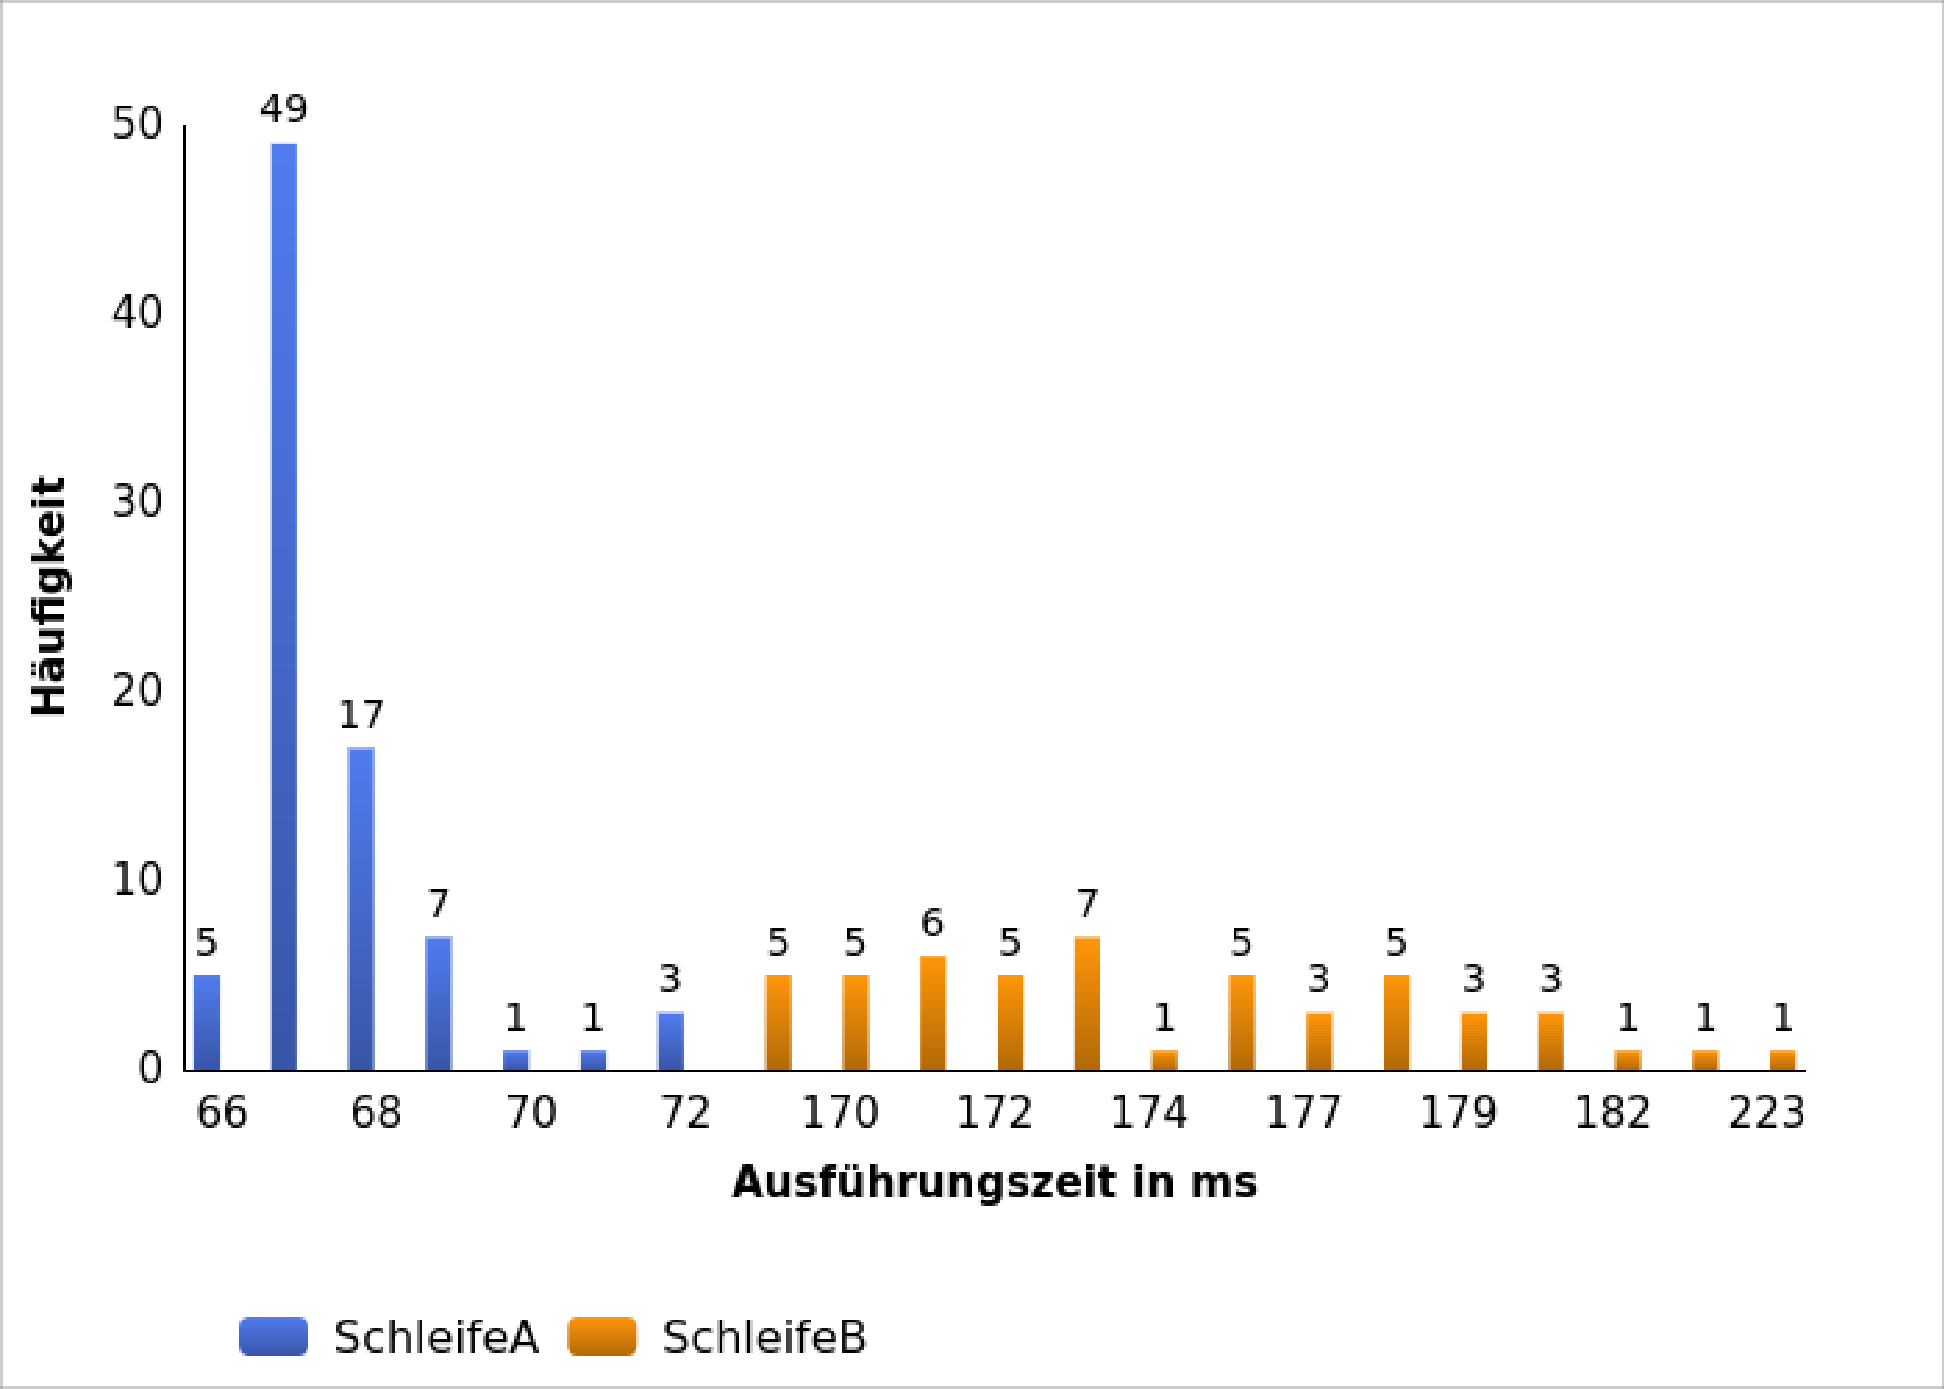
\includegraphics[width=\linewidth]{./image/ausfuehrungszeit-einfach.pdf}
    %\subsection{1. Lösungsansatz}
    %+einfach zu implementieren, da wir kein schleifenkonstrukt mehr benötigen.
    %+keine Endlosschleife, weil es keine Schleifen gibt
    %+keine Zyklen, weil der Ablauf linear ist
    %+weniger Sprünge, weil keine for oder while Bedingungen vorhanden sind
    %+möglicher Performance gewinn, weil Schleifen-Overhead entfällt
    %-größerer Codeumfang, da der eigentliche schleifenkörper a-mal im code implemtniert werden muss 
    %-höherer verbraucht an ressourcen zB Speicher mehr code = mehr speicher
    %-möglicherweise ineffizient, wenn der faktor zu groß gewählt wird
    %-schlechtere Lesbarkeit
    %-wenn bereits nach 3 durchlaufen feststeht, dass das gewünschte ergbeniss nicht mehr erreicht werden kann werden trotzdem die restlichen schritte ausgeführt
    %\subsection{2. Lösungsansatz}
    %+keine Endlosschleife, weil maximale Schleifendurchläufe begrenzt sind.
    %+
    %-azyklisches verhalten wird verletzt, weil schleifenkonstrukt benötigt wird
    %-
    \newpage
    \chapter{Ausblick}
    %TODO treshold, robustheit dass block a mit 1,6k iterationen arbeiten kann, visualisierung dass ergebnisse nicht eingetroffen ist
    In diesem Kapitel werden mögliche Weiterentwicklung und zukünftige Forschungsarbeiten beschrieben. 
    Die erst im späten Verlauf aufgetreten sind oder aus Zeitgründen nicht bearbeitet werden konnten.
    Der Threhsold für den Algorithmus Block B wird aktuell fest in den Code implementiert werden. 
    Das sollte in der Praxis so nicht sein. 
    Hier würde es sich anbieten einen Algorithmu zu entwerfen der den Threshold dynmaisch anpasst jenachdem welche Eingabe er bekommt.
    Ein anderer Punkt, ist dass derBneutzer aktuell kein Feedback bekommt, ob ein Ergebniss gefunden wurden ist oder nicht.
    Um das zu verbessern könnte eine Meldung ins System implementiert werden, wenn der Algorithmus nicht durchgeht, dass der Benutzer eine Meldung bekommt, dass keine Lösung gefunden werden konnte.\\
    Ein anderer Punkt der verbessert werden kann, ist die Robustheit des Block A. 
    Dieser führt aktuell bei einer großen Anzahl an Iterationen zu einen Overflow. 
    aus
    \newpage
    \renewcommand{\refname}{}
    \chapter{Literaturverzeichnis}
    \begin{thebibliography}{9}
        \bibitem{2}Johnston, W., Hanna, J., \& Millar, R. (2004). \emph{Advances in dataflow programming languages}. ACM Computing Surveys, 36(1), 1–34.
        \bibitem{3}Chen, L. (2021). \emph{Iteration vs. Recursion: Two Basic Algorithm Design Methodologies}. SIGACT News, 52(1), 81–86.
        \bibitem{4}Arvind, \& Culler, D. (1986). \emph{Dataflow Architectures}. LCS Technical Memos.
        \bibitem{5}Ambler, A., \& Burnett, M. (1990). \emph{Visual forms of iteration that preserve single assignment}. Journal of Visual Languages \& Computing, 1(2), 159–181.
        \bibitem{6}Mosconi, M., \& Porta, M. (2000). \emph{Iteration constructs in data-flow visual programming languages}. Computer Languages, 26(2), 67–104.
        \bibitem{1}Fan, Z., Li, W., Liu, T., Tang, S., Wang, Z., An, X., Ye, X., \& Fan, D. (2022). \emph{A Loop Optimization Method for Dataflow Architecture}. In 2022 IEEE 24th Int Conf on High Performance Computing \& Communications; 8th Int Conf on Data Science \& Systems; 20th Int Conf on Smart City; 8th Int Conf on Dependability in Sensor, Cloud \& Big Data Systems \& Application (HPCC/DSS/SmartCity/DependSys) (pp. 202–211).
        \bibitem{7}Gévay, G., Soto, J., \& Markl, V. (2021). \emph{Handling Iterations in Distributed Dataflow Systems}. ACM Comput. Surv., 54(9), 199:1–199:38.
        \bibitem{8}Alves, T., Marzulo, L., Kundu, S., \& França, F. (2021). \emph{Concurrency Analysis in Dynamic Dataflow Graphs}. IEEE Transactions on Emerging Topics in Computing, 9(1), 44–54.
        \bibitem{9}Ye, Z., \& Jiao, J. (2024). \emph{Loop Unrolling Based on SLP and Register Pressure Awareness}. In 2024 20th International Conference on Natural Computation, Fuzzy Systems and Knowledge Discovery (ICNC-FSKD) (pp. 1–6).
        \bibitem{10}Lučanin, D., \& Fabek, I. (2011). \emph{A visual programming language for drawing and executing flowcharts}. In 2011 Proceedings of the 34th International Convention MIPRO (pp. 1679–1684).
        \bibitem{11}Davis, A., \& Keller, R. (1982). \emph{Data Flow Program Graphs}. All HMC Faculty Publications and Research.
        \bibitem{21}Boshernitsan, M., \& Downes, M. (2004). \emph{Visual Programming Languages: A Survey}. EECS University of California, Berkeley.
        \bibitem{12}Charntaweekhun, K., \& Wangsiripitak, S. (2006). \emph{Visual Programming using Flowchart}. In 2006 International Symposium on Communications and Information Technologies (pp. 1062–1065).
        \bibitem{13}Burnett, M., Baker, M., Bohus, C., Carlson, P., Yang, S., \& Van Zee, P. (1995). \emph{Scaling up visual programming languages}. Computer, 28(3), 45–54.
        \bibitem{14}Kurihara, A., Sasaki, A., Wakita, K., \& Hosobe, H. (2015). \emph{A Programming Environment for Visual Block-Based Domain-Specific Languages}. Procedia Computer Science, 62, 287–296.
        \bibitem{15}Hils, D. (1992). \emph{Visual languages and computing survey: Data flow visual programming languages}. Journal of Visual Languages \& Computing, 3(1), 69–101.
        \bibitem{19}Sousa, T. (2012). \emph{Dataflow Programming Concept, Languages and Applications}. Doctoral Symposium on Informatics Engineering, 7.
        \bibitem{18}Van Deursen, A., Klint, P., \& Visser, J. (2000). \emph{Domain-specific languages: an annotated bibliography}. ACM SIGPLAN Notices, 35(6), 26–36.
        \bibitem{16}Roy, G., Kelso, J., \& Standing, C. (1998). \emph{Towards a visual programming environment for software development}. In Proceedings. 1998 International Conference Software Engineering: Education and Practice (Cat. No.98EX220) (pp. 381–388). IEEE Comput. Soc.
        \bibitem{20}Weintrop, D. (2019). \emph{Block-based programming in computer science education}. Communications of the ACM, 62(8), 22–25.
        \bibitem{22}Gumm, H.P., \& Sommer, M. (2016). \emph{Band 1 Programmierung, Algorithmen und Datenstrukturen}. De Gruyter Oldenbourg.
    \end{thebibliography}
\end{document}    